\documentclass[runningheads]{llncs}

\usepackage[export]{adjustbox}
\usepackage{algorithm}
\usepackage{algpseudocode}
\usepackage{amsmath}
\usepackage{amssymb}
\usepackage[english]{babel}
\usepackage{bbm}
\usepackage{bm}
\usepackage{booktabs}

\usepackage{csquotes}

\usepackage{float}
\usepackage[letterpaper,top=2cm,bottom=2cm,left=3cm,right=3cm,marginparwidth=1.75cm]{geometry}

\usepackage[acronym,section=section]{glossaries}

\usepackage{graphicx}

\usepackage[backref=page, colorlinks=true, allcolors=blue]{hyperref}

\usepackage{cleveref}

\usepackage{mathrsfs}
\usepackage{mathtools}
\usepackage{microtype}
\usepackage{subfig}
\usepackage{tikz}

\usetikzlibrary{external}
\usetikzlibrary{positioning}
\tikzexternalize[prefix=assets/,figure name=architecture]

\DeclareMathOperator*{\argmax}{arg\,max}
\DeclareMathOperator*{\argmin}{arg\,min}

\setlength{\tabcolsep}{8pt}

\makeglossaries

\newacronym{ai}{AI}{Artificial Intelligence}
\newacronym{dqn}{DQN}{Deep Q-Network}
\newacronym{iqm}{IQM}{interquartile mean}
\newacronym{lstm}{LSTM}{Long Short-Term Memory}
\newacronym{mdp}{MDP}{Markov decision process}
\newacronym{ml}{ML}{Machine Learning}
\newacronym{mse}{MSE}{mean squared error}
\newacronym{ngu}{NGU}{NeverGiveUp}
\newacronym{per}{PER}{Prioritized Experience Replay}
\newacronym{r2d2}{R2D2}{Recurrent Replay Distributed DQN}
\newacronym{rl}{RL}{Reinforcement Learning}
\newacronym{rnn}{RNN}{Recurrent Neural Network}
\newacronym{sota}{SOTA}{state-of-the-art}
\newacronym{td}{TD}{temporal-difference}
\newacronym{tqn}{TQN}{Transformer Q-Network}
\newacronym{ucb}{UCB}{Upper-Confidence-Bounds}


\begin{document}

\title{Investigating the benefits of adding self-attention \break to a Deep Q-Network}

\author{Roberto Schiavone\inst{1}\orcidID{0009-0001-9167-1496} \\
\email{r.schiavone@vu.nl}}

\authorrunning{R. Schiavone}

\institute{Vrije Universiteit Amsterdam, De Boelelaan 1105,  1081 HV Amsterdam, The Netherlands}

\maketitle

\begin{abstract}

In recent years, the Transformer architecture has revolutionized how we process sequential data, but its applications in online \acrshort{rl} settings are still very limited. In this paper a Transformer architecture is applied as the first layer inside a \acrshort{dqn} in order to process in parallel a set of observations. The hypothesis is that the encoder-decoder architecture can extract more information from an observation than a linear layer. Furthermore, the multi-head attention can help the network focus on what experiences are deemed most important. In the end I provide detailed results, backed by a recently suggested statistical framework, to show that the proposed architecture surpasses the baseline on 1 of the 3 classic control environments used for evaluation, but on average it performs worse, providing a good starting point for future research.

\keywords{Reinforcement Learning \and Transformers \and Classic control}
\end{abstract}

\section{Introduction}
\acrfull{rl} is the field of \acrlong{ai} that focuses on training an intelligent agent to make sequential decisions in an environment in order to maximize a specific goal or reward. It is inspired by how humans and animals learn through trial and error, by taking actions and receiving feedback. The agent does not know \textit{a priori} which actions to take, but it must instead discover the ones that yield the highest reward by trying them. In some cases, actions affect not only the immediate reward but also the next state and, through that, all subsequent rewards \cite{rlbook,rlbook2}.

Unfortunately, despite the progresses made in the field, pioneered by the seminal works on Deep \acrlong{rl} \cite{dqn1,dqn2}, \acrshort{rl} is ridden with problems that still make it an unfeasible paradigm for most \acrfull{ml} tasks. \acrshort{rl} is sample inefficient, requiring hundreds of millions of steps for benchmarks such as the Atari Learning Environment (ALE) \cite{atari}, corresponding to tens to hundreds of hours of human play experience \cite{rldoesntwork,rainbow}. Good reward functions that encourage the actual wanted behavior are difficult to design, and prone to fail in unexpected ways \cite{rldoesntwork,concrete_problems_in_ai_safety}; the final results are unstable and hard to reproduce due to random chance generating too much variance, and thus playing a major role during training \cite{drl_that_matters,rldoesntwork}. Randomness can also lead the agents to get stuck in local optima from which it is nigh-on-impossible to escape for the rest of the training phase \cite{rldoesntwork}.

In recent years, the Transformer architecture has reshaped the landscape of \acrshort{ai}, since it is extremely well-suited for applications that deal with sequential data, such as Natural Language Processing \cite{gpt2,gpt3} and Computer Vision \cite{swin_transformer}. By being able to process sequences as a whole rather than token by token, Transformers do not suffer from long dependency issues and do not have to deal with past information, since there are no past states to account for.

In this paper I explore the impact of using a Transformer architecture as the first layer of a \acrfull{dqn}, and I train it on chosen toy environments in the context of online\footnote{In an online setting, instead of relying on previously collected data, the agent explores the environment and it collects experiences by actively interacting with it.}, off-policy\footnote{The agent learns not only from the current interaction, but only from previous interactions that have been gathered with a different policy.} learning. The key idea behind it is that a set of observations can be seen as a sequence on which a Transformer architecture can be trained. Furthermore, the multi-head attention mechanism can help capture what experiences from the set are the most important.

In the end I show that the architecture I propose, called \acrfull{tqn}, is not only able to learn and converge to the optimal policy over time, but it is also able to yield a higher score than the baseline on 1 of the 3 chosen environments. The results are further corroborated following the statistical framework proposed by \texttt{rliable} \cite{rliable}.

\section{Related Work}

\subsection{Transformers in Offline \acrshort{rl}}

\subsubsection{Trajectory Transformer}
\sloppy The Trajectory Transformer trains on sequences of transitions $(state, action, reward)$ and it repurposes beam search as a reward-maximizing strategy \cite{trajectory_transformer}. The Decision Transformer, explained below, is an improved iteration of the Trajectory transformer.

\subsubsection{Decision Transformer}
Decision Transformers are able to learn meaningful patterns from a dataset of previously gathered experiences. A linear layer embeds each token, which is then augmented with information about the current timestep. Lastly, a Generative Pretrained Transformer (GPT) model predicts the future actions. By leveraging a causally masked Transformer, the model exceeds the performance of previous \acrfull{sota} offline \acrshort{rl} baselines for Atari, OpenAI Gym, and Key-to-Door tasks \cite{decision_transformer}. My approach draws inspiration from the Decision Transformer, but it differs in the implementation and how it is applied to online learning instead.

\subsubsection{Q-Transformer}
Q-Transformer is the latest architecture for offline Q-learning with a Transformer
model, only one month old at the moment of writing. The Q-Transformer architecture discretizes the action space and uses an autoregressive model update to avoid the curse of dimensionality on the discretized actions. The encoding of each observation is concatenated with the embeddings from the previous predicted action and it is then processed by Transformer layers. One-hot action vectors are used to predict the Q-values of the next actions. The architecture adopts Conservative Q-learning (CQL) to minimize the over-estimation of Q-values.\cite{q_transformer}. Q-Transformer is the latest offline \acrshort{rl} architecture that successfully uses a Transformer to improve the performance of Q-learning, and it beats the Decision Transformer on all the previously mentioned benchmarks.

\subsection{State of the Art: MEME}

\subsubsection{\acrfull{r2d2}}
R2D2 incorporates a \acrfull{lstm} into an $n$-step, dueling \acrshort{dqn} with a prioritized distributed replay in order to capture temporal dependencies in the data. A \acrfull{lstm} layer after the convolutional one and an aggressive approach in experience prioritization help achieve a better performance than Rainbow \cite{r2d2}. The \textit{stored state} training strategy stores experiences from different agents in an experience replay that is subsequently fed to the agent, the \textit{burn-in} strategy uses a portion of the experiences to bring the network to the starting training state \cite{r2d2}. \acrshort{r2d2} is one of the earliest and most successful examples to explicitly use a layer for sequential data, in this case a \acrshort{lstm}.

\subsubsection{\acrfull{ngu}}
\acrshort{ngu} adds to the approach proposed by \acrshort{r2d2} an a universal value function approximator to approximate the optimal value function. The model introduces a Retraced Q-learning loss function, and it distributes training in order to collect a large amount of experiences from parallelized environments \cite{never_give_up}. \acrshort{ngu} encourages the agent to continue exploring the environment, hence the name, even if it encounters difficulties, so that the agent can learn better policies. \acrshort{ngu} combines curiosity-driven exploration with distributed \acrshort{rl} agents; the model is the cornerstone for Agent57 \cite{agent57}.

\subsubsection{Agent57}
Agent57 splits the state-action value function in two different components, with different parameterized sets of weights, to train two neural networks sharing the same architecture. As a result, the training stability significantly improves. Furthermore, Agent57 introduces the \textit{meta-controller} as a mechanism to select the best policy during training \cite{agent57}.

\subsubsection{MEME}
MEME builds upon the previous 3 architectures, \acrshort{r2d2}, \acrshort{ngu} and Agent57. The model introduces a trust region to determine which samples contribute to the loss, employs a variation of the NFNet architecture to stabilize the network without using layer normalization, and achieves more robust behavior through policy distillation\footnote{Policy distillation is the transfer of knowledge from a more complex policy to a simpler one, allowing the simpler policy to learn and perform well while reducing at the same time the computational complexity of training it.} \cite{meme}. I find it worth mentioning MEME because, at the moment of writing, it is the state of the art for online \acrshort{rl} on the Atari benchmark.

\begin{figure}[!htbp]
\centering
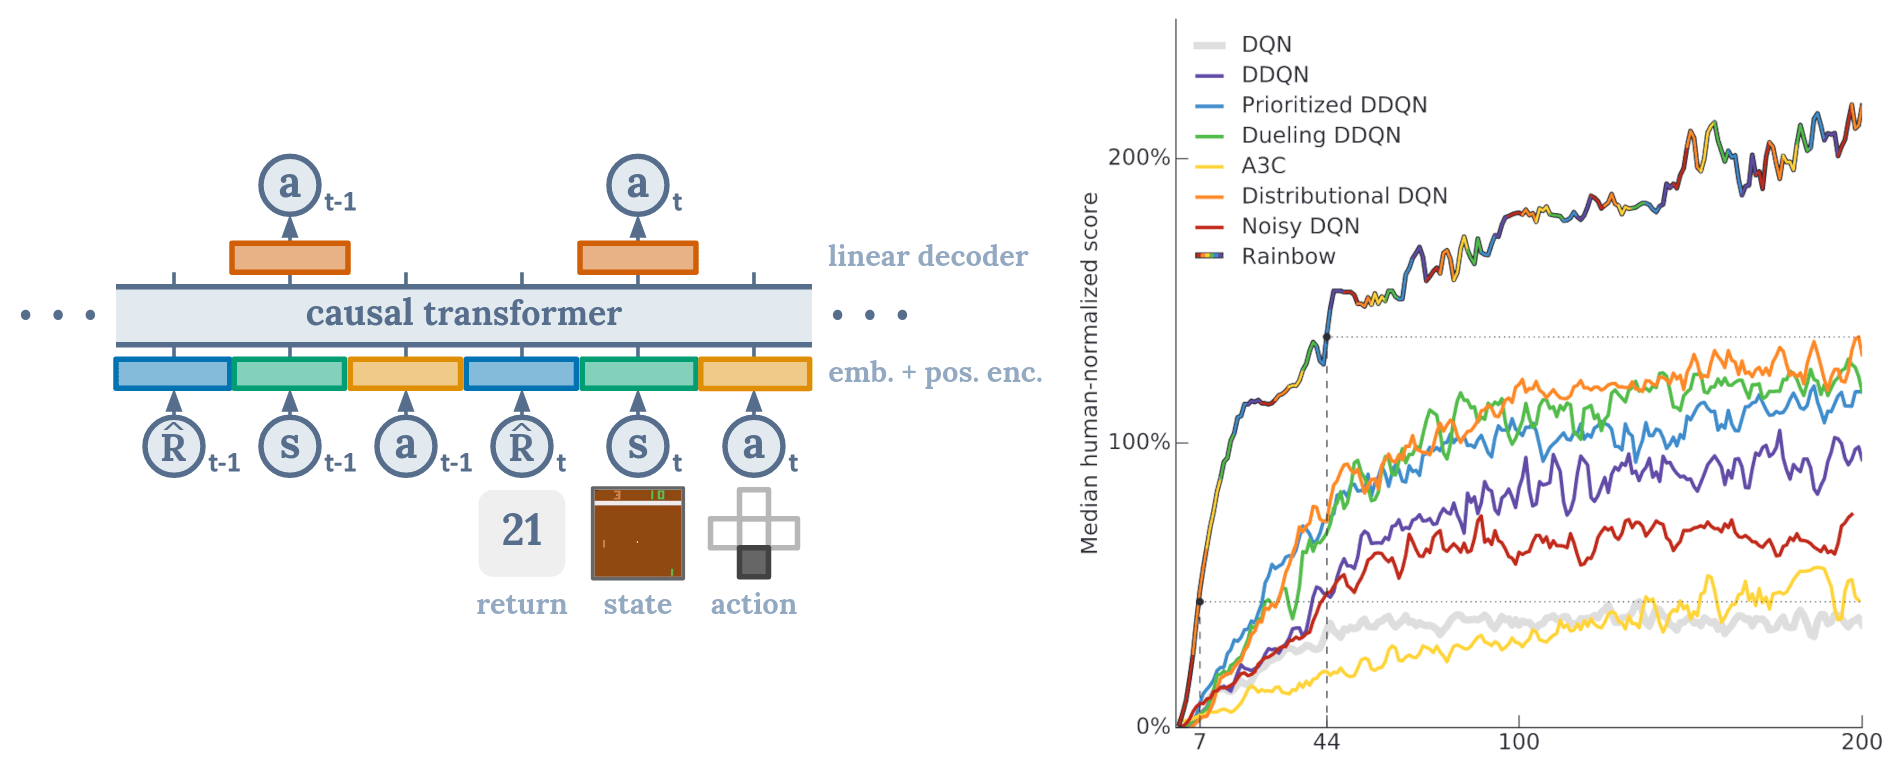
\includegraphics[width=\textwidth]{images/decision-transformer-rainbow.png}
\caption{On the left, the Decision Transformer architecture \cite{decision_transformer}. On the right, Rainbow (discussed later, see \nameref{subsec:rainbow}) performance on the Atari benchmark compared to its single components \cite{rainbow}.}
\label{fig:rainbow}
\end{figure}

\section{Background}

\subsection{\acrlong{rl}}
\acrshort{rl} is the area of \acrfull{ml} that deals with sequential decision-making. In a \acrshort{rl} setting, an agent interacts with the environment through trial-and-error approach and, for each action taken, it receives either a positive or negative reward as unique feedback. The agent doesn't know \textit{a priori} which actions to take, but it must instead discover the ones that yield the highest reward by trying them. In some cases, actions affect not only the immediate reward but also the next state and, through that, all subsequent rewards \cite{rlbook,rlbook2}.

The sequence of actions and observations, $s_t = x_1, a_1, x_2, \dots, a_{t-1}, x_t$, can be modeled as a \acrfull{mdp} in which each sequence is a distinct state; the algorithm converges to the optimal action-value function by using the Bellman equation in an iterative update \cite{rlbook,rlbook2,dqn1}.

\subsection{\acrlong{mdp}}
An \acrshort{mdp} \cite{mdp} is a 5-tuple $(\mathcal{S}, \mathcal{A}, \mathcal{P}_a, \mathcal{R}_a, \gamma)$, where:
\begin{itemize}
    \item $\mathcal{S}$ is a finite set of states called the \textit{state space},
    \item $\mathcal{A}$ is a finite set of actions called the \textit{action space},
    \item $\mathcal{P}_a = P(s_{t+1} = s' \mid s_t = s, a_t = a)$ is the probability that action $a$ in state $s$ at time $t$ will lead to state $s'$ at time $t+1$,
    \item $\mathcal{R}_a(s, s')$ is the reward received after transitioning from state $s$ to state $s'$, due to action $a$,
    \item $\gamma \in [0, 1]$ is a discount factor.
\end{itemize}

\subsection{Bellman equation}
For a given policy $\pi$ and a state $s$ and action $a$ in the \acrshort{mdp}, the Bellman equation for state-action values (Q-values) is defined as follows \cite{mdp}:

$$
Q_\pi(s, a) = \sum [P(s' \mid s, a) * (R(s, a, s') + \gamma * \sum [\pi(a' \mid s') * Q_\pi(s', a')])]
$$

\begin{itemize}
    \item $Q_\pi(s, a)$: the expected cumulative reward (Q-value) of taking action $a$ in state $s$ and then following policy $\pi$.
    \item $P(s' \mid s, a)$: the probability of transitioning to state $s'$ from state $s$ when taking action $a$.
    \item $R(s, a, s')$: the immediate reward received when transitioning from state $s$ to state $s'$ by taking action $a$.
    \item $\gamma$: the discount factor.
    \item $\pi(a' \mid s')$: the probability of taking action $a'$ in state $s'$ according to policy $\pi$.
\end{itemize}

\subsection{Exploration vs. Exploitation}
In an offline \acrshort{rl} setting, an agent merely learns from a dataset of experiences separately obtained. In online \acrshort{rl} problems instead, an agent has to face the peculiar exploration-exploitation dilemma. During training, the agent must choose whether to explore more states in order to discover a better policy, or to exploit the information already available to maximize the reward in the short term, but risk being stuck in a local optimum. The exploration-exploitation problem is not fully solved and various partial solutions have been proposed throughout the years. Below, I present a non-exhaustive list of the most used approaches.

\subsubsection{Epsilon-Greedy}
In an $\epsilon$-greedy policy, a parameter $\epsilon$ determines the action taken by the agent. If a random number sampled from a continuous uniform distribution $\mathcal{U}(0, 1)$ is less than $\epsilon$, then the agent takes a random action to explore the environment, otherwise it exploits its knowledge of the environment by taking the action that in the past yielded the best results.

$\epsilon$-greedy is the most used policy because it is easy to understand, but in some cases it is not the most efficient. Furthermore, it is difficult to find the best value for $\epsilon$ depending on the task. A commonly adopted tactic is to linearly or exponentially decrease $\epsilon$ over time by an extra parameter $\epsilon_{\text{decay}}$. Thus, the agent performs more explorations of the environment at the beginning of the training, and takes less random actions further down the road. For this paper, $\epsilon$-greedy is the most relevant approach because it is used in \nameref{subsec:deep_q_learning}.

\subsubsection{Thompson sampling and \acrfull{ucb}}
Thompson sampling is a heuristic where the action is chosen by drawing it from a probability distribution over possible values of unknown parameters. It then chooses the action assuming that the sampled values are the true ones, and over time it adjusts the probability distribution according to the feedback received from the environment \cite{thompson}.

\acrshort{ucb} is another strategy used in online \acrshort{rl} with partial information feedback. Compared to Thompson sampling, \acrshort{ucb} takes a deterministic approach instead. Taking into consideration an action's expected reward and a confidence interval representing its uncertainty, an upper confidence bound is computed for each action, then the one with the highest upper confidence bound is chosen. This way the agent is encouraged to choose an exploratory action by selecting the one with the highest uncertainty.

\subsubsection{Boltzmann distributions}
Another approach is to model the probabilities of choosing the different actions with a Boltzmann distribution. A temperature parameter $\tau$ controls the level of randomness; a higher temperature means a more uniform distribution, making it easier to choose a random action, while a lower temperature pushes the agent to exploit the actions that are deemed better.

\subsubsection{Adding noise}
The last approach worth mentioning that is used to balance exploration-exploitation is to add noise to the current observation (see also \nameref{subsec:rainbow}). By adding noise to its inputs, the actions taken from the agent are less deterministic, thus encouraging exploration.


\subsection{Q-learning}
Q-learning is an off-policy \acrshort{td} control algorithm defined by \cite{qlearning}

$$
Q(s, a) \leftarrow Q(s, a) + \alpha \left[R(s, a, s') + \gamma \max_a Q(s', a) - Q(s, a)\right].
$$

In this case, the learned action-value function $Q$ directly approximates $q_*$, the optimal action-value function, independent of the policy being followed.

\subsection{Deep Q-learning} \label{subsec:deep_q_learning}
Deep Q-learning is a variant of Q-learning where the model is a convolutional neural network. The input of the neural network is the state of the environment, and the output is a value function estimating future rewards \cite{dqn2}.

The network is trained  with stochastic gradient descent to update the weights. To alleviate the problems of correlated data and non-stationary distributions, an experience replay is introduced \cite{dqn1}.

\begin{algorithm}
\caption{Deep Q-Learning with Experience Replay \cite{dqn1,dqn2}}
\label{algo:dqn}
\begin{algorithmic}
\State Initialize replay memory $\mathcal{D}$ to capacity $N$
\State Initialize action-value function $Q$ with random weights
\For {episode $ = 1, M$}
\State Initialize sequence $s_1 = \{ x_1 \}$
\For {$t = 1, T$}
\State With probability $\epsilon$ select a random action $a_t$
\State otherwise select $a_t = \max_a Q^*(s_t, a; \theta)$
\State Set $s_{t+1} = s_t, a_t, x_{t+1}$
\State Store transition $(s_t, a_t, r_t, s_{t+1})$ in $\mathcal{D}$
\State Sample random minibatch of transitions $(s_j, a_j, r_j, s_{j+1})$ from $\mathcal{D}$
\State Set $ y_j =
\begin{cases}
r_j &\text{for terminal } \phi_{j+1} \\
r_j + \gamma \max_{a'} Q(\phi_{j+1}, a'; \theta) &\text{for non terminal } \phi_{j+1}
\end{cases}
$
\State Perform a gradient descent step on $(y_j - Q(s_j, a_j; \theta))^2$
\EndFor
\EndFor
\end{algorithmic}
\end{algorithm}

\subsection{Chasing Rainbows} \label{subsec:rainbow}
\subsubsection{Double \acrshort{dqn}} \label{subsubsec:double_dqn}
Double \acrshort{dqn} is an extension of \acrshort{dqn} designed to address the overestimation problem present in the Q-learning algorithm and DQN. Using two separate networks, one for action estimation and one for evaluation, reduces overestimation and improves overall performance \cite{double_dqn}.

In a double \acrshort{dqn} setting, given a minibatch of transitions $(s_j, a_j, r_j, s_{j+1})$ from replay memory $\mathcal{D}$, the target is updated as follows \cite{rainbow}:

\begin{equation}
\label{eq:double_dqn}
(R_{t+1} + \gamma_{t+1} q_{\bar\theta}(S_{t+1}, \argmax_{a'} q_\theta(S_{t+1}, a')) - q_\theta(S_t, A_t))^2.    
\end{equation}

\subsubsection{\acrfull{per}}
A standard experience replay memory samples previous transitions uniformly. Prioritizing which transitions are replayed makes experience replay more efficient and effective. Transitions with a bigger \acrfull{td} error have a higher priority; stochastic prioritization and importance sampling alleviate the introduced bias and loss of diversity \cite{prioritized_experience_replay}.

The probability $p_t$ is the probability of sampling a transition relative to the the last encountered absolute \textit{\acrshort{td} error}:

\begin{equation}
\label{eq:per}
    p_t \propto \lvert R_{t+1} + \gamma_{t+1} \max_{a'} q_{\bar\theta}(S_{t+1}, a') - q_\theta(S_t, A_t) \rvert^\omega,
\end{equation}

where $\omega$ is a hyperparameter that determines the shape of the distribution \cite{rainbow}.

\subsubsection{Dueling \acrshort{dqn}}
A dueling \acrshort{dqn} explicitly separates the representation of state values and action advantages in two separate functions. The two streams, representing the dueling architecture, share a common feature layer \cite{dueling_dqn}.

The new action values are computed as following:

\begin{equation}
\label{eq:dueling_dqn}
q_\theta(s, a) = v_\eta (f_\xi(s)) + a_\psi (f_\xi(s), a) - \frac{\sum_{a'} a_\psi(f_\xi(s), a')}{N_{\text{actions}}}
\end{equation}

where $\xi$, $\eta$ and $\psi$ are, respectively, the parameters of the shared encoder $f_\xi$, of the value stream $v_\eta$, and of the advantage stream $a_\psi$; ${ \theta = \{ \xi, \eta, \psi \} }$ is their concatenation \cite{rainbow}.

\subsubsection{$n$-step learning}
A multi-step variant of \acrshort{dqn} is defined by minimizing the alternative loss \cite{n_step_learning}

\begin{equation}
\label{eq:n_step_learning}
(R_t^{(n)} + \gamma_t^{(n)} \max_{a'} q_{\bar\theta}(S_{t+n},a') - q_\theta(S_t, A_t))^2, \quad \text{where } R_t^{(n)} = \sum_{k=0}^{n-1} \gamma_t^{(k)} R_{t+k=+1}.
\end{equation}

\subsubsection{Distributional \acrshort{dqn}}
Instead of learning the expected return, the network can be trained to learn the distribution of returns \cite{distributional_dqn}:

\begin{equation}
\label{eq:distributional_dqn}
d'_t \equiv (R_{t+1} + \gamma_{t+1} \bm z, \bm p_{\bar\theta}(S_{t+1}, \bar{a}^*_{t+1})), D_{\text{KL}} (\Phi_{\bm z} d'_t \Vert d_t),
\end{equation}

\sloppy where $\Phi_{\bm z}$ is a L2-projection of the target distribution onto the fixed support $\bm z$, and ${ \bar{a}^*_{t+1} = \argmax_a q_{\bar\theta}(S_{t+1}, a) }$ is the greedy action with respect to the mean action values ${ q_{\bar\theta}(S_{t+1}, a) = \bm z^\intercal \bm p_\theta(S_{t+1}, a) }$ in state $S_{t+1}$ \cite{rainbow}.

\subsubsection{NoisyNet}
NoisyNet enhances the \acrshort{dqn} weights with parametric noise. The added stochasticity, over time, aids the network to ignore the noise over time, allowing the network to perform a more efficient exploration. The parameters of the noise are learned over time, and the added noise removes the need of the hyperparameter $\epsilon$, that determines the ratio between exploration and exploitation \cite{noisy_net}.

The noisy stream is computed as following:

\begin{equation}
\label{eq:noisy_net}
\bm y = (\bm b + \bm Wx) + (\bm b_{\text{noisy}} \odot \epsilon^b + (\bm W_{\text{noisy}} \odot \epsilon^w) \bm x),
\end{equation}

where $\epsilon^b$ and $\epsilon^w$ are random variables, and $\odot$ denotes the element-wise product \cite{rainbow}.

\subsubsection{Rainbow}
Rainbow is an integrated agent that combines approaches from \textbf{Eq.}~\ref{eq:double_dqn} to \textbf{Eq.}~\ref{eq:noisy_net} and adds them to \textbf{Alg.}~\ref{algo:dqn}. The result algorithm beats the previous \acrshort{sota} performance on the Atari 2600 benchmark \cite{rainbow}. Some components of Rainbow, such as Double DQN and the \acrlong{per} are reused and compared later on in the \nameref{section:method} section.

\subsection{Transformers}
A Transformer model is composed of an encoding part connected to a decoding part. The encoding part is made of multiple encoder layers stacked on top of each other; each encoder processes its input through a self-attention layer, which enables it to consider other parts of the sequence as it encodes each input. The output of the self-attention layer becomes then the input of a feed-forward neural network \cite{attention_is_all_you_need}. The result of the encoding layers is added to the original sequence to create a more refined understanding of the input.

\begin{figure}[!htbp]
\centering
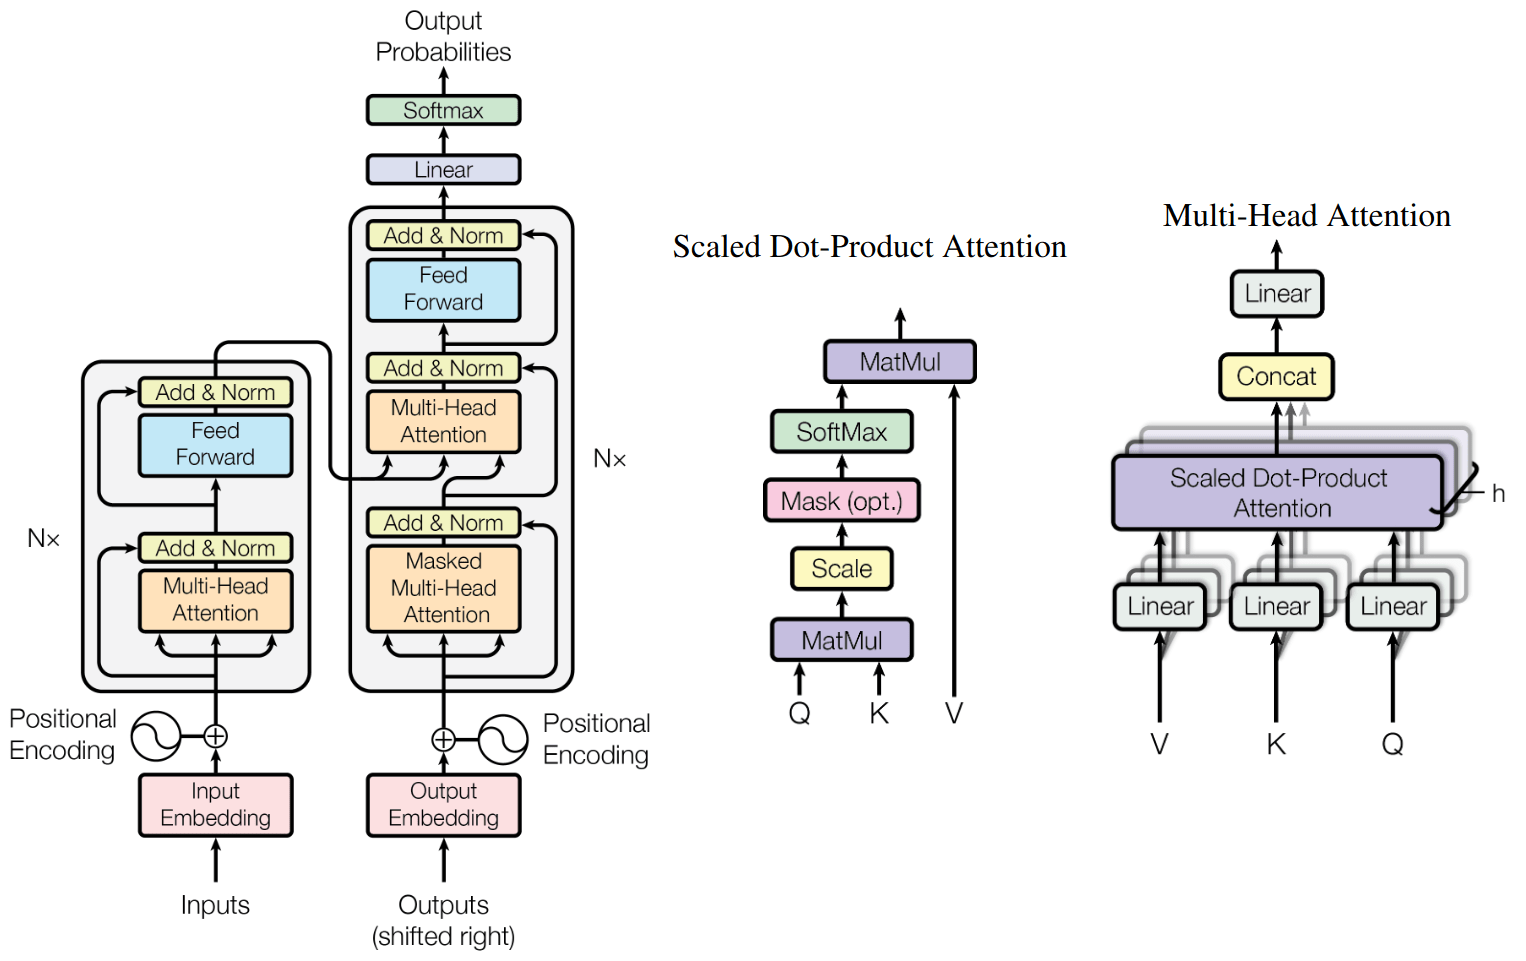
\includegraphics[width=\textwidth]{images/transformer.png}
\caption{From left to right: the Transformer architecture, the Scaled Dot-Product Attention and the Multi-Head Attention, consisting of several attention layers running in parallel \cite{attention_is_all_you_need}.}
\label{fig:transformer}
\end{figure}

The decoding part shares the same structure of the encoding part, but each decoder adds, between the self-attention and the feed-forward layer, an extra attention layer that helps the decoder focus on the important parts of the input sequence \cite{attention_is_all_you_need}.

The Transformer architecture has strong generalization capabilities, it is more efficient than sequential models since it is able to process sequential data in parallel, and it is easy to scale to large amounts of data. 

\subsubsection{Embedding} 
In a Transformer architecture, each element is mapped to a unique embedding. The purpose of embedding is to provide the model with information about what each token of the input sequence represents. Through this process the model can find over time better and better representations for the input.

Since Transformers process sequential data in parallel, they do not have a representation of the order of the inputs in the sequence. Positional encoding adds information about where each element is in the sequence; some common approaches include adding a sinusoidal function to the input sequence or to learn the encoding from scratch during training.

\subsubsection{The Attention Mechanism}
First introduced by \cite{seq2seq}, the attention mechanism allows the model to ``pay attention" to the different parts of the input sequence in order to learn which parts are more relevant for the final prediction. For each element of the input sequence, the attention mechanism computes a score that indicates its importance for the current prediction. The score is computed by taking into account the context and other relevant information from the input sequence. Elements with higher scores contribute more to the final prediction.

\section{Method} \label{section:method}

The intuition behind the \acrshort{tqn}, shared by the related work on offline \acrshort{rl} \cite{decision_transformer,q_transformer}, is that a set of observations, on which the network is trained, can be seen as a sequence, for which the Transformer architecture is particularly suited.

By replacing the first layer of a \acrshort{dqn} with a Transformer layer, the neural network can extract more relevant features, and the multi-head attention mechanism is trained to recognize the more relevant observations from the set, without the added complexity of a \acrshort{per}. However, this happens on a smaller scale, since \acrshort{per} samples the most important experiences from the entire experience replay, while the multi-head attention chooses the most relevant experiences from a smaller set of observations.

The expected result can become a viable way to increase stability during training and to improve performance, leading to a quicker convergence to the optimal policy.

\subsection{Baseline}
The input to the neural network consists of a tensor containing the state of the environment. The neural network processes the input through  two hidden layers consisting of $256$ units, both followed by a rectifier nonlinearity. The output layer is a linear layer whose values are the predicted Q-values for each individual action, given the input state \cite{dqn1,dqn2}. Each layer of the neural network is a fully-connected layer (see \textbf{Fig.}~\ref{fig:dqn-architecture}. In order to reduce over-estimation, a copy of the network is used to evaluate the predictions (see \nameref{subsubsec:double_dqn}).

\begin{figure}[!htbp]
\tikzset{
  every neuron/.style={
    circle,
    draw,
    minimum size=1cm
  },
  neuron missing/.style={
    draw=none, 
    scale=4,
    text height=0.333cm,
    execute at begin node=\color{black}$\vdots$
  },
}
\centering
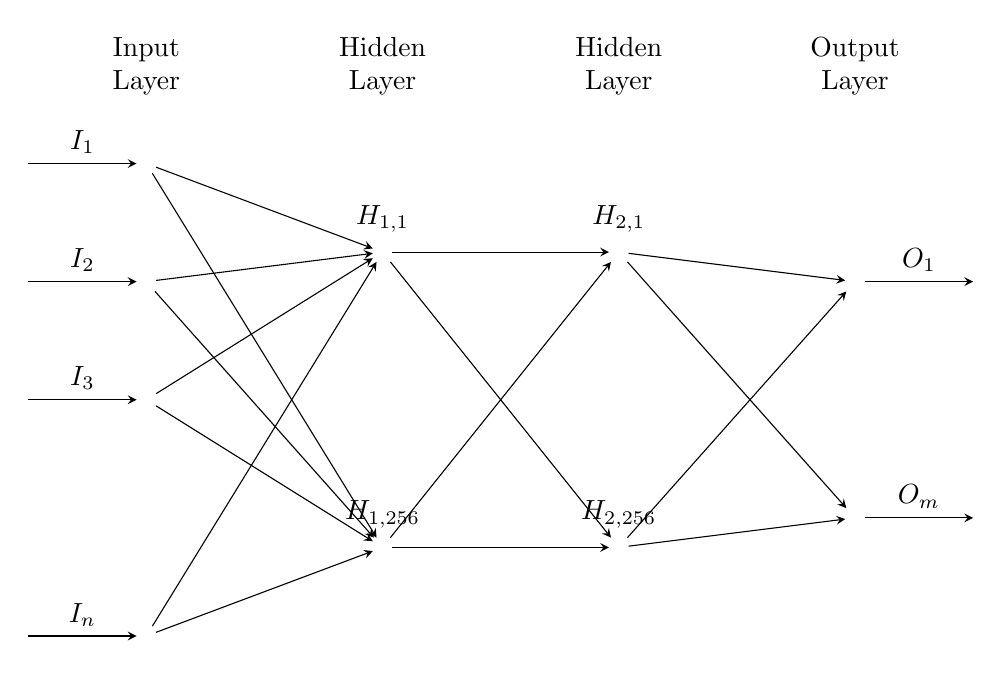
\begin{tikzpicture}[x=1.5cm, y=1.5cm, >=stealth]

\foreach \m/\l [count=\y] in {1,2,3,missing,4}
  \node [every neuron/.try, neuron \m/.try] (input-\m) at (0,2.5-\y) {};

\foreach \m [count=\y] in {1,missing,2}
  \node [every neuron/.try, neuron \m/.try ] (hidden1-\m) at (2,2-\y*1.25) {};

\foreach \m [count=\y] in {1,missing,2}
  \node [every neuron/.try, neuron \m/.try ] (hidden2-\m) at (4,2-\y*1.25) {};

\foreach \m [count=\y] in {1,missing,2}
  \node [every neuron/.try, neuron \m/.try ] (output-\m) at (6,1.5-\y) {};

\foreach \l [count=\i] in {1,2,3,n}
  \draw [<-] (input-\i) -- ++(-1,0)
    node [above, midway] {$I_\l$};

\foreach \l [count=\i] in {1,256}
  \node [above] at (hidden1-\i.north) {$H_{1,\l}$};

\foreach \l [count=\i] in {1,256}
  \node [above] at (hidden2-\i.north) {$H_{2,\l}$};

\foreach \l [count=\i] in {1,m}
  \draw [->] (output-\i) -- ++(1,0)
    node [above, midway] {$O_\l$};

\foreach \i in {1,...,4}
  \foreach \j in {1,...,2}
    \draw [->] (input-\i) -- (hidden1-\j);

\foreach \i in {1,...,2}
  \foreach \j in {1,...,2}
    \draw [->] (hidden1-\i) -- (hidden2-\j);

\foreach \i in {1,...,2}
  \foreach \j in {1,...,2}
    \draw [->] (hidden2-\i) -- (output-\j);

\foreach \l [count=\x from 0] in {Input, Hidden, Hidden, Output}
  \node [align=center, above] at (\x*2,2) {\l \\ Layer};

\end{tikzpicture}
\caption{The \acrlong{dqn} architecture.}
\label{fig:dqn-architecture}
\end{figure}

\subsection{Transformer Q-Network}

The Transformer Q-Network consists instead of an encoding component, a decoding component, followed by two hidden fully-connected layers and the output layer. Both the encoding and decoding components also stack two hidden layers each, all sharing the same parameters. Each encoder/decoder layer has an input and output size equal to the observation size, with a hidden layer of size $256$. The dropout value is set to $0.1$ and the attention heads are set equal to the observation size, which can be  $4$, $6$ or $8$ depending on the environment.


\begin{figure}[H] 
\centering
\subfloat{%
\resizebox{0.35\textwidth}{!}{
\tikzset{
  every neuron/.style={
    circle,
    draw,
    minimum size=1cm
  },
  neuron missing/.style={
    draw=none, 
    scale=4,
    text width=0.333cm,
    execute at begin node=\color{black}$\ldots$
  },
}
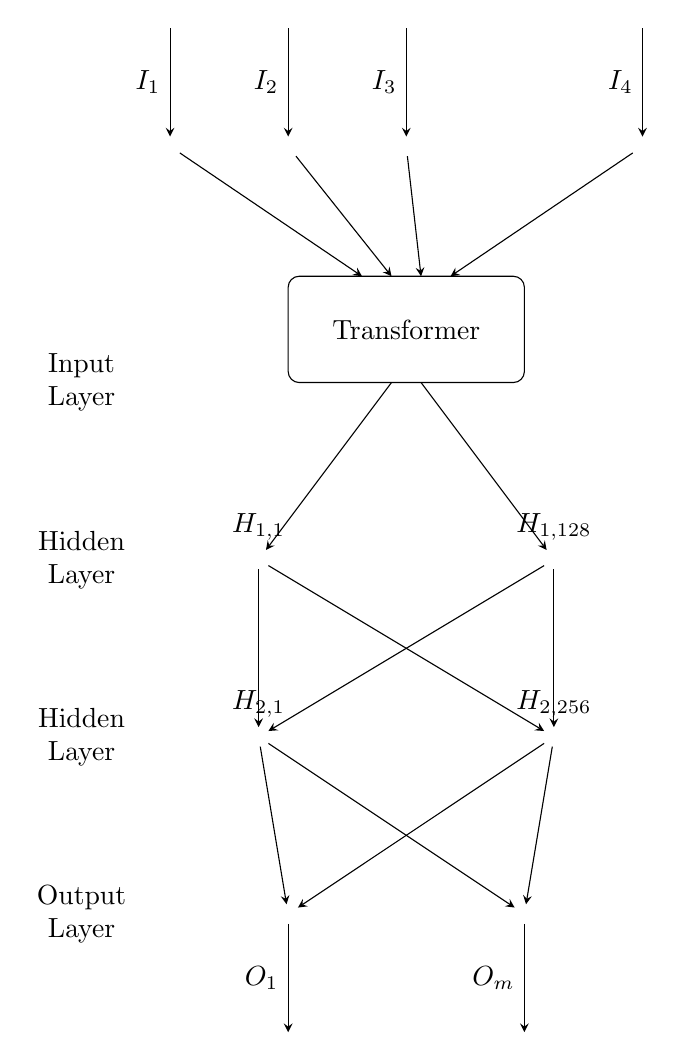
\begin{tikzpicture}[x=1.5cm, y=1.5cm, >=stealth]%
  
\foreach \m/\l [count=\x] in {4,missing,3,2,1}
  \node [every neuron/.try, neuron \m/.try] (input-\m) at (0.25-\x, 6.5) {};

\draw [rounded corners] (-3.75,4.5) rectangle (-1.75,5.4);
\node [anchor=center] at (-2.75,4.95) {Transformer};

\foreach \m [count=\x] in {1,missing,2}
  \node [every neuron/.try, neuron \m/.try ] (hidden1-\m) at (-0.25-\x*1.25,3) {};

\foreach \m [count=\x] in {1,missing,2}
  \node [every neuron/.try, neuron \m/.try ] (hidden2-\m) at (-0.25-\x*1.25,1.5) {};

\foreach \m [count=\x] in {1,missing,2}
  \node [every neuron/.try, neuron \m/.try ] (output-\m) at (-0.75-\x,0) {};

\foreach \l [count=\i] in {1,2,3,4}
  \draw [<-] (input-\i) -- ++(0,1)
    node [midway, left] {$I_\l$};

\foreach \l [count=\i] in {128, 1}
  \node [above] at (hidden1-\i.north) {$H_{1,\l}$};

\foreach \l [count=\i] in {256, 1}
  \node [above] at (hidden2-\i.north) {$H_{2,\l}$};

\foreach \l [count=\i] in {m,1}
  \draw [->] (output-\i) -- ++(0,-1)
    node [midway, left] {$O_\l$};

\foreach \i in {1,...,4}
    \draw [->] (input-\i) -- (-3.375 + 0.25*\i,5.4);

\def\hiddenlist{{2,1}}
\foreach \i [evaluate=\i as \y using {\hiddenlist[\i-1]}] in {1,...,2} {
    \draw [->] (-3.125 + 0.25*\i,4.5) -- (hidden1-\y);
}

\foreach \i in {1,...,2}
  \foreach \j in {1,...,2}
    \draw [->] (hidden1-\i) -- (hidden2-\j);

\foreach \i in {1,...,2}
  \foreach \j in {1,...,2}
    \draw [->] (hidden2-\i) -- (output-\j);

\foreach \l [count=\y from 0] in {Output, Hidden, Hidden, Input}
  \node [align=center] at (-5.5,\y*1.5) {\l \\ Layer};

\end{tikzpicture}%
}%
}%
\hfill%
\subfloat{%
\raisebox{1.5cm}[0pt][0pt]{%
\makebox[0.64\textwidth][c]{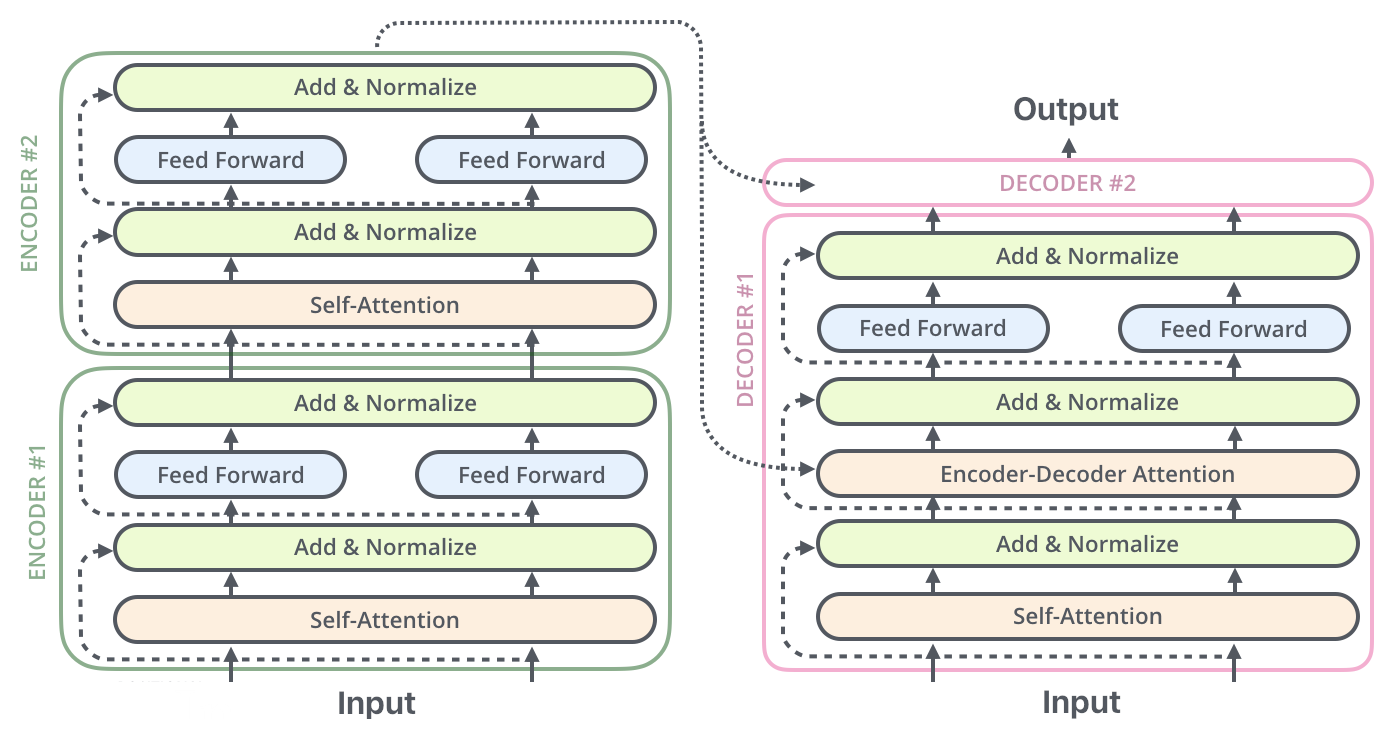
\includegraphics[width=0.64\textwidth]{images/exploded-encoder-decoder.png}}%
}%
}%
\caption[On the left, a simplified view of the \acrlong{tqn}. On the right, the inner components of the Transformer layer. Image on the right adapted from ``The Illustrated Transformer".]{On the left, a simplified view of the \acrlong{tqn}. On the right, the inner components of the Transformer layer. Image on the right adapted from ``The Illustrated Transformer"\protect\footnotemark.}
\label{fig:tqn-architecture}
\end{figure}

\footnotetext{\url{https://jalammar.github.io/illustrated-transformer/}}


First, the batch of observations gets reshaped to a single batch, containing a sequence of observations, the previous batch size is now the length of the sequence. The encoder/decoder pair extracts the relevant features from the observation, then the two fully-connected hidden layers of size $128$ and $256$, respectively, process it further. Each linear layer is always followed by a rectifier nonlinearity activation function. Finally, the output layer is again a linear layer whose values are the predicted Q-values for each possible action.


\subsection{A Note on Embedding}
Embedding is used with the attention model to transform a discrete token of the input sequence in a continuous vector representation. For the chosen environments, the observation is already in the form of a vector of floating point numbers, therefore preprocessing it through an embedding layer is not needed.

Depending on the task, before embedding a sequence, each token may be augmented with positional encoding. Again, this step was deemed not needed for two reasons: the sequence is not going through an embedding layer, and each observation does not temporally come after the previous one, but it is independently sampled from the experience replay. Preliminary iterations of the network that also employed an embedding step had the score over time collapse towards the worst possible value with no sign of recovery.

\begin{algorithm}
\caption{\textbf{Baseline}: Double DQN with Experience Replay \cite{dqn1,dqn2,double_dqn}}
\label{alg:baseline}
\begin{algorithmic}
\State Initialize replay memory $\mathcal{D}$ to capacity $N$
\State Initialize action-value function $Q$ with random weights
\For {episode $ = 1, M$}
\State Initialize sequence $s_1 = \{ x_1 \}$
\For {$t = 1, T$}
\State With probability $\epsilon$ select a random action $a_t$
\State otherwise select $a_t = \max_a Q^*(s_t, a; \theta)$
\State Set $s_{t+1} = s_t, a_t, x_{t+1}$
\State Store transition $(s_t, a_t, r_t, s_{t+1})$ in $\mathcal{D}$
\State Sample random minibatch of transitions $(s_j, a_j, r_j, s_{j+1})$ from $\mathcal{D}$
\State Set $ y_j =
\begin{cases}
r_j &\text{for terminal } s_{j+1} \\
r_{j+1} + \gamma Q(s_{t+1}, \argmax_{a} Q(s_{j+1}, a; \theta); \theta_{\text{target}}) &\text{for non-terminal } s_{j+1}
\end{cases}
$
\State Perform a gradient descent step on $(y_j - Q(s_j, a_j; \theta))^2$
\EndFor
\EndFor
\end{algorithmic}
\end{algorithm}

\section{Experimental Setup}

Both the baseline and the new \acrshort{tqn} architecture are implemented from scratch in Python with PyTorch \cite{pytorch}. The flow of the code follows the previous work done by CleanRL \cite{cleanrl}, the logic is encapsulated in classes similar to ``Rainbow Is All You Need" \cite{rainbow_is_all_you_need} and the hyperparameters share the same naming convention as Stable-Baselines 3 \cite{sb3}.

Despite being more complex, the \acrshort{tqn} has fewer parameters than the \acrshort{dqn}, $49k$ vs $68k$.

\subsection{Environments}
Although all three are considered toy environments, these environments are chosen with the following criteria in mind. First of all, all of them have a continuous observation space represented by a vector of \texttt{float}, and all of them expect, at each step, a single discrete action. Therefore, the neural network architecture does not need changes to adapt to the environments.

Interestingly, they are all different, each in their own way, because of the way their reward function is defined. \textit{Acrobot} always returns a fixed negative reward, \textit{CartPole} always returns a fixed positive reward, and \textit{LunarLander} provides a \textit{shaped reward} function that returns every time a different positive or negative value, depending on the state of the lander.

\begin{figure}[H]
\centering
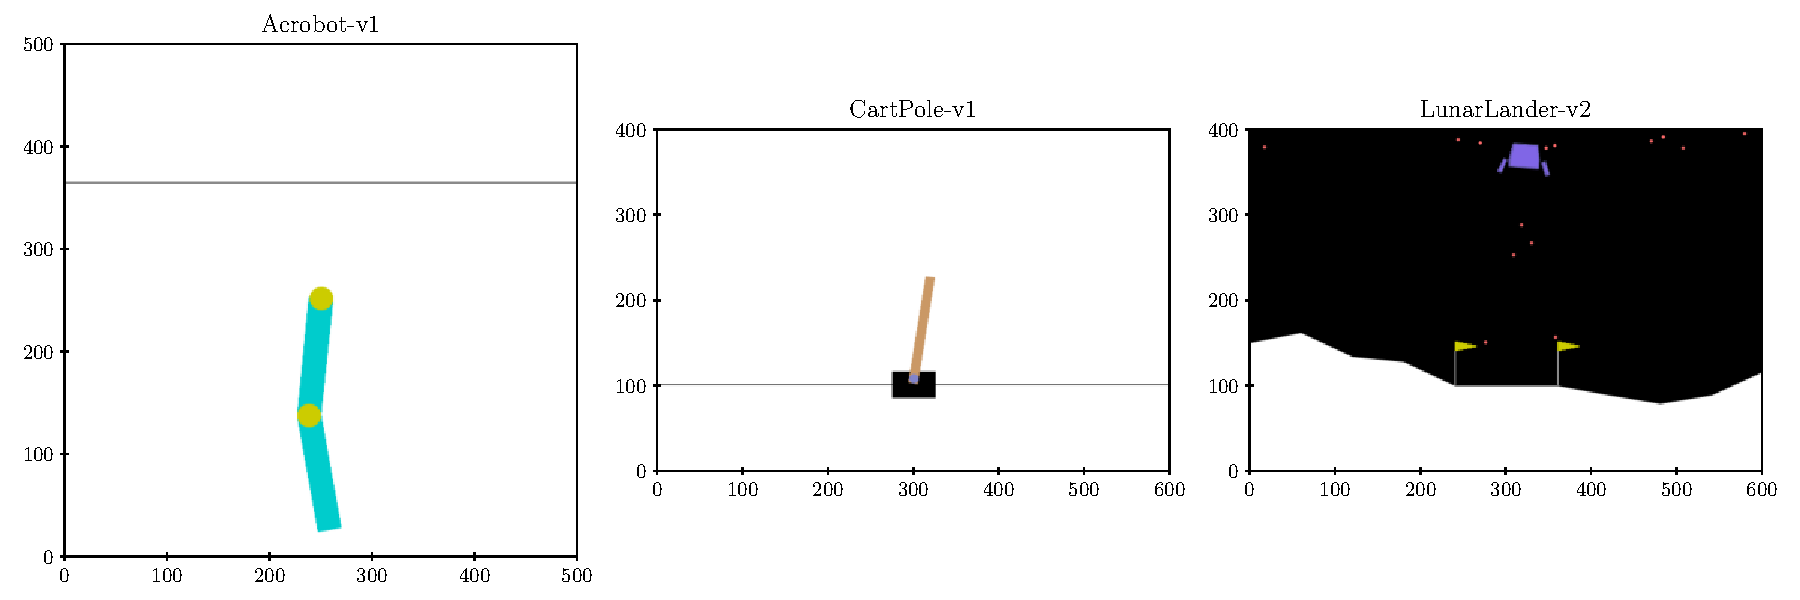
\includegraphics[width=\textwidth]{images/environments.pdf}
\caption{Example screenshots for each environment. From left to right: Acrobot, CartPole, LunarLander.}
\label{fig:environments}
\end{figure}

\subsubsection{Acrobot}
The Acrobot is a two-link under-actuated robot, an arm with the first joint fixed in place, and the joint between the two links actuated \cite{acrobot}.

The observation contains the values of the $\sin$ and $\cos$ of the two joints, and their respective angular velocities. The three possible actions are applying positive torque, negative torque, and no torque to the actuated joint. The objective is to swing the other end above the bar by an amount equal to the length of one of the links. The reward is $-1$ for each step taken and an episode ends if the robot either reaches the bar or takes the maximum number of allowed steps. An episode is considered successful if it reaches a reward threshold of $-100$ \cite{farama_gymnasium}.

A reward function that provides a fixed negative reward at each step, regardless of the state, is easy to design and pushes the agent to find its way to the target in the shortest possible amount of time. Conversely, the agent relies on the reward as a feedback on how good/bad the action taken is, and since the reward does not change, the agent may not have sufficient information to distinguish the good actions from the bad ones.

\subsubsection{CartPole}
The CartPole is a cart to which a rigid pole is hinged on its center. The cart moves on a frictionless track and the pole starts from an upright position \cite{cartpole}.

At each step, the available information about the environment is the cart position and linear velocity, and the pole angle and its angular velocity. The agent has no control on the pole, but it can push the cart left or right instead. Despite being discrete actions, the velocity is modeled depending on the angle of the pole. The reward is $+1$ for each step taken and the objective is to keep the pole upright for as long as possible. An episode terminates if the maximum score of $500$ is reached, if the cart goes beyond the edges of the frame, or if the pole is too tilted \cite{farama_gymnasium}.

Similar to \textit{Acrobot}, the CartPole agent receives a constant reward at each step taken, but this time it is a positive $+1$. Again, the agent cannot rely on the reward to gauge the optimality of its actions, but instead the implicit target is to keep the episode running for as long as possible.

\subsubsection{LunarLander} \label{subsubsec:lunar_lander}
The LunarLander environment is a rocket trajectory optimization problem. The lander has infinite fuel and it can either run the engines at full throttle or turn them off \cite{openai_gym}.

The observation provides information about the position of the lander in the space, the linear $x$ and $y$ velocities, its tilt, its angular velocity and whether or not each of the legs has touched the ground. The possible actions the lander can take are either be idle, or fire the engines (left, main or right respectively). The reward is modulated according to the distance from the landing pad, its speed and its tilt. An additional reward of $\pm 100$ is assigned after either landing safely or crashing \cite{farama_gymnasium}.

Since the reward function for the LunarLander provides a \textit{shaped reward}, the agent is able to learn faster and make quick adjustments to its policy since it receives immediate feedback for each action taken. A shaped reward function better informs the agent on its closeness to the target but, at the same time, it is more difficult to design, and it may be exploited in unexpected ways. For example, instead of learning to land safely (in which case it would receive maximum reward), the LunarLander agent may learn to hover just above the landing pad because in that state it also receives a reward close to the maximum.

\subsection{Loss and Parameter Optimization}
To represent how well the predicted values align with the target values, I use the \acrfull{mse}, which is the average of the squared difference between two values:

$$
\ell(x, y) = \bar{L}, \quad L = \{ l_1, \dots, l_N \}^\intercal, \quad l_n = (x_n - y_n)^2,
$$

where $N$ is the batch size, $x$ and $y$ are tensors of $n$ elements each.

The Adam optimizer takes care of adapting the learning rate to each network parameter individually. The parameters with more significant gradients are updated according to a smaller effective learning rate, while parameters with smaller gradients get a larger effective learning rate. Furthermore, Adam optionally adds weight decay as a regularization technique that penalizes large weights during training \cite{adam}, but in this case it is not used.

The optimizer updates the weights according to the following logic:

$$
\theta_t \leftarrow \theta_{t-1}  - \alpha \cdot \hat{m}_t / (\sqrt{\hat{b}_t} + \omega),
$$

where $\theta_t$ is the updated weight, $\theta_{t-1}$ is the current weight, $\alpha$ is the learning rate, $\hat{m}_t$ is the biased first moment estimate, $\hat{b}_t$ is the biased second raw moment estimate, and $\omega$ is a small constant for numerical stability \cite{adam}.

\subsection{Algorithm Hyperparameters}
Although different in the implementation from Stable-Baselines 3 \cite{sb3}, I choose to use the same hyperparameter names in most of the cases.

Optimal hyperparameters for \acrshort{dqn} are taken from \texttt{rl-baselines3-zoo} \cite{rl_zoo3}; the same set of hyperparameters is used for \acrshort{tqn}. Every episode rollout is capped at a maximum of $500$ steps.

\begin{table}[!htbp]
\caption{Hyperparameters used across all runs.}
\label{table:hyperparameters}
\centering
\begin{tabular}{@{} r c c c @{}}
\toprule
& \textbf{Acrobot-v1} & \textbf{CartPole-v1} & \textbf{LunarLander-v2} \\
\midrule
max steps                   & 100.000 &  50.000 & 100.000 \\
gradient clip               &         &    10.0 &         \\
accumulate gradient batches &         &       1 &         \\
batch size                  &     128 &      64 &     128 \\
learning rate               &  6.3e-4 &  2.3e-3 &  6.3e-4 \\
buffer size                 &  50.000 & 100.000 &  50.000 \\
learning starts             &       0 &   1.000 &       0 \\
tau                         &         &     1.0 &         \\
gamma                       &         &    0.99 &         \\
train frequency             &       4 &     256 &       4 \\
gradient steps              &         &       1 &         \\
target update interval      &     250 &      10 &     250 \\
exploration fraction        &    0.12 &    0.16 &    0.12 \\
epsilon max                 &         &     1.0 &         \\
epsilon min                 &     0.1 &    0.04 &     0.1 \\
\bottomrule
\end{tabular}
\end{table}

\begin{itemize}
    \item \textit{max steps}: total number of environment steps to train on;
    \item \textit{gradient clip}: maximum value for the gradient clipping of the network parameters;
    \item \textit{accumulate gradient batches}: gradient steps to take before updating the policy; 
    \item \textit{batch size}: minibatch size for each policy update;
    \item \textit{learning rate}: how much the policy weights should be updated w.r.t. the loss gradient;
    \item \textit{tau}: soft update coefficient, if $\tau = 1$ a hard update is performed instead;
    \item \textit{gamma}: discount factor;
    \item \textit{train frequency}: steps to perform between each policy update;
    \item \textit{target update interval}: environment steps to take between each target network update;
    \item \textit{exploration fraction}: fraction of entire training period over which the exploration rate is reduced; e.g. if the max steps are $100.000$ and the exploration fraction is $0.12$, $\epsilon$ linearly decreases from $\epsilon_{\max}$ to $\epsilon_{\min}$ during the first $12.000$ steps; 
    \item \textit{epsilon max}: exploration factor, initial probability of taking a random action;
    \item \textit{epsilon min}: exploration factor, final probability of taking a random action.
\end{itemize}

\subsection{Network Hyperparameters Tuning}
For the \acrshort{tqn}, I use a trial-and-error approach to find the best hyperparameters to make the network learn and converge. I only focus on tuning the parameters of the new network architecture; the default \texttt{nn.Transformer}\footnote{\url{https://pytorch.org/docs/stable/generated/torch.nn.Transformer.html}} parameters ($6$ encoder layers, $6$ decoder layers, and $2048$ units for each hidden layer) provided by PyTorch are, computationally-wise, prohibitively expensive.

As a first step, I progressively decrease the number of layers until it is possible to train the network on a consumer GPU. On the GPU worker I used for training, the default Transformer parameters grind the iterations to a halt, the computation time explodes from mere minutes to hours, with sudden crashes of the system as a result of out-of-memory errors. I end up fixing the size of the encoder and decoder components to $2$ layers each.

I then focus on the size of the hidden encoder/decoder layers. $2048$ units are too much for such a simple input, and they destabilize the network. The model is too complex and it starts performing poorly on new observations. A very large hidden layer is also prone to the exploding or vanishing gradient problem. For this reason, I set the units of each hidden layer to $256$. This proves to be sufficient for the network to converge.

Lastly, I investigate the impact of the number of heads in this multi-head attention model. Setting it to $1$ brings the worst results during training; this is expected because a single attention head is not enough to capture the different  relationships and the more complex dependencies within the data. Setting the number of attention heads equal to $2$ already bring better results, but empirically the best results come by setting them equal to the size of the observation, $4$, $6$ and $8$ depending on the environment.

\section{Results and Discussion}

For each run, I gather data such as loss, Q-values, episode reward and episode length; $\epsilon$ over time is also collected for debug purposes, but it is left out of the analysis because it is simply linearly annealed from $\epsilon_{\max}$ to $\epsilon_{\min}$ for each environment step for a total of \textit{max steps} $\times$ \textit{exploration fraction}, with no extra logic applied to it. Each model is trained on $20$ different fixed seeds (see \textbf{\nameref{section:appendix_c}}). I then interpolate the results of each run so that I can compute the mean of each episode. In order to denoise the mean score per episode, I also compute a smoothed version of the obtained line, a rolling average with $n = \frac{\text{number of episodes}}{10}$.

Despite being the most simple environment, none of the networks are able to learn to balance the pole in the \textit{CartPole} environment, and the \acrshort{tqn} fails to find a successful policy for \textit{Acrobot}. Supplementary analysis for these environments is relegated to the \textbf{\nameref{section:appendix_c}}. 

\begin{table}[H]
\label{table:results-LunarLander-v2}
\caption{Performance of the models tested across all the environments.}
\centering
\begin{tabular}{@{} r c c c c c c @{}}
\toprule
& \multicolumn{2}{c}{Acrobot-v1} & \multicolumn{2}{c}{CartPole-v1} & \multicolumn{2}{c}{LunarLander-v2} \\
\midrule
& $R_{\;mean}$ & $R_{\;best}$ & $R_{\;mean}$ & $R_{\;best}$ & $R_{\;mean}$ & $R_{\;best}$ \\
\midrule
DQN & \textbf{-91.99} & \textbf{-61} & \textbf{77.54} & 281.00 & \textbf{151.88} & 317.45 \\
TQN & -490.26 & -72 & 38.03 & \textbf{500} & 46.3 & \textbf{322.74} \\
\bottomrule
\end{tabular}
\end{table}

For the analysis, I take as a reference the \textit{LunarLander} environment, since it is the only one where both architectures converge. For the LunarLander environment, an episode is considered a valid solution if it scores $200$ points or more.

For the most relevant metrics I use \textbf{bootstrapping with stratified sampling} to compute the $95\%$ \textbf{confidence intervals}; the bootstrapping uses $50.000$ replications \footnote{The process of repeatedly sampling with replacement from the underlying data in order to create a simulated dataset.}; the sample efficiency curve normalizes the scores between $0$ and the target score $\tau = 200$.

\begin{figure}[!htbp]
\centering
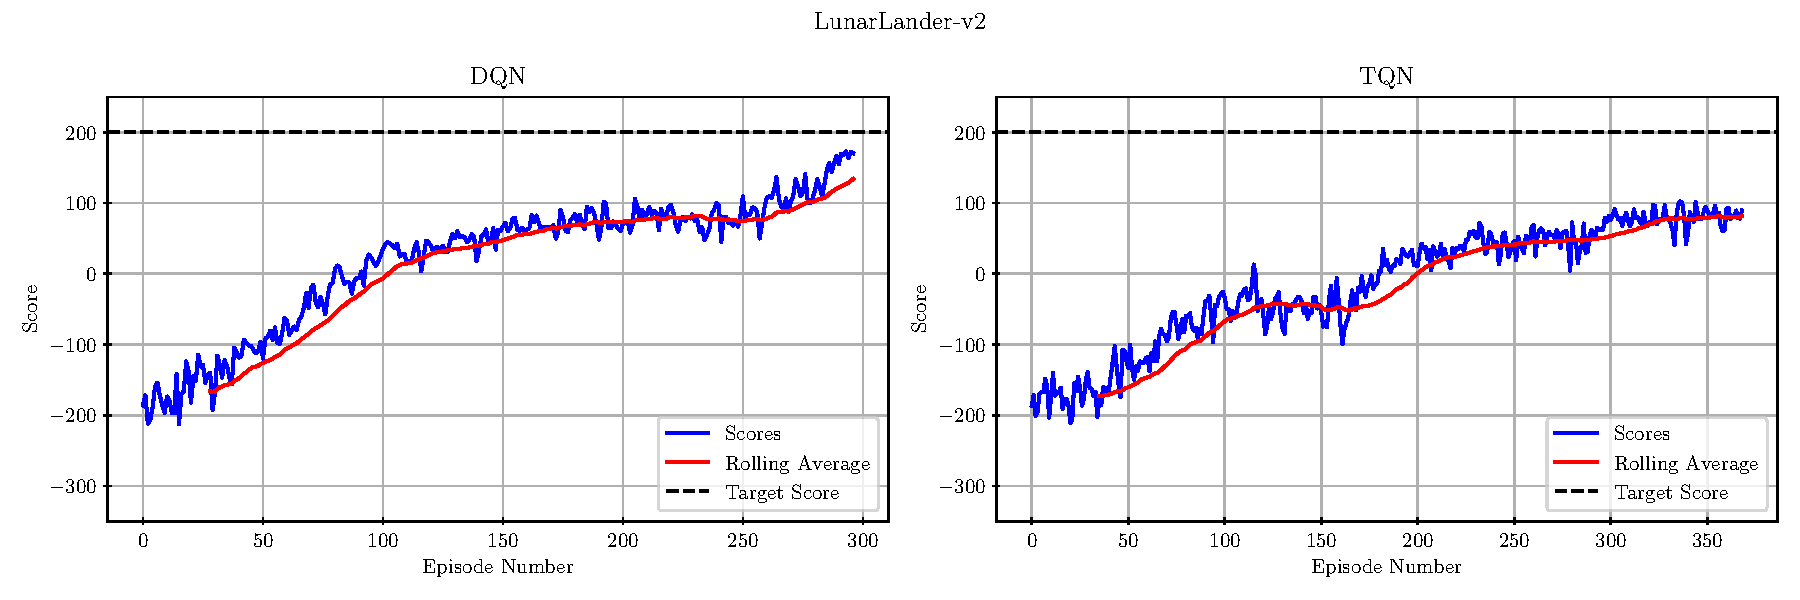
\includegraphics[width=\textwidth]{images/score-vs-episode_DQN-TQN_LunarLander-v2.pdf}
\caption{Each run has the same number of environment steps but, since the episode length is not fixed, the total number of episodes may differ.}
\label{fig:score-vs-episode-LunarLander-v2}
\end{figure}

In \textbf{Fig.}~\ref{fig:score-vs-episode-LunarLander-v2}, both sample efficiency curves have the shape of a logarithmic curve showing peak efficiency towards the end of the training and approaching the target score of $200$, but \acrshort{tqn} performs worse and has a higher variance. The new architecture shows convergence to the optimal policy over time, but from the plot it may seem that it is less efficient than the baseline. In reality, when I consider the the confidence intervals of the \textbf{\acrfull{iqm}}, the performance on the middle $50\%$ of the combined runs computed by removing the top and bottom $25\%$ of the runs \cite{rliable}, the probability of improvement shows that the \acrshort{tqn} performs better than the baseline (see \textbf{Fig.}~\ref{fig:sample-efficiency-LunarLander-v2}). The \textbf{probability of improvement} is a metric that shows how likely it is for $X$ to outperform $Y$ on a randomly selected task, where 

\begin{equation}
P(X > Y) = \frac{1}{M} \sum^M_{m=1} P(X_m > Y_m),
\label{eq:probability_of_improvement}
\end{equation}

with $P(X_m > Y_m)$ the probability of $X$ being better than $Y$ at task $m$ \cite{rliable}.

In this case, $P(\acrshort{dqn} > \acrshort{tqn}) = 0.48$, which is equivalent to say $P(\acrshort{tqn} > \acrshort{dqn}) = 0.52$, meaning that, given a random task, the \acrlong{tqn} gets a better reward than the baseline $52\%$ of the time.

\begin{figure}[!htbp]
\centering
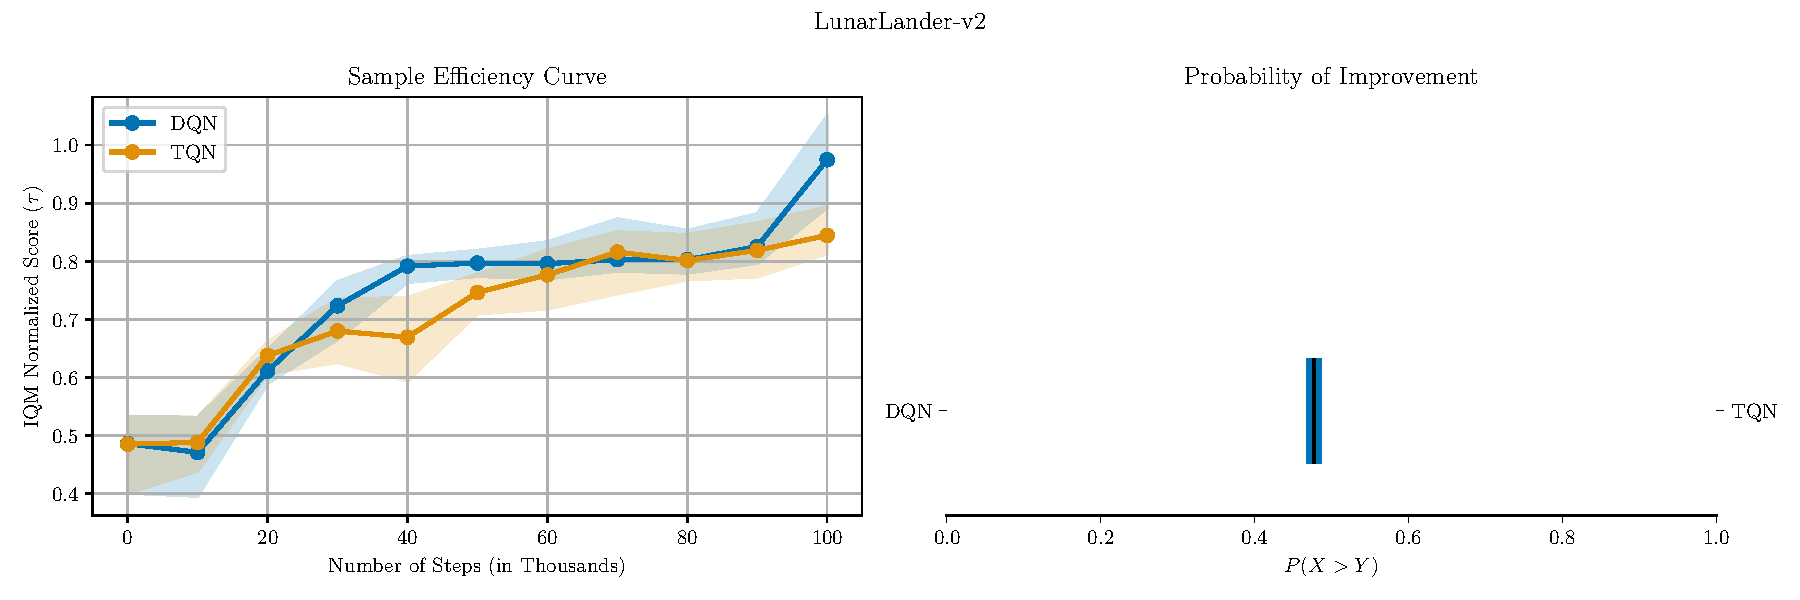
\includegraphics[width=\textwidth]{images/sample-efficiency-probability-improvement_DQN-TQN_LunarLander-v2.pdf}
\caption{On the left, sample efficiency of agents as a function of number of steps measured via \acrshort{iqm} scores. Shaded regions show pointwise 95\% percentile stratified bootstrap CIs, as suggested by \cite{rliable}. On the right, the probability of improvement.}
\label{fig:sample-efficiency-LunarLander-v2}
\end{figure}

To check whether each model has over-confident Q-values, I average the results of $400$ test runs for each architecture ($20$ models, $1$ for each seed, play environments tested with all the seeds). For a consistent range of comparison, both the rewards and Q-values gathered this way are normalized between $-1$ and $1$.

\begin{figure}[!htbp]
\centering
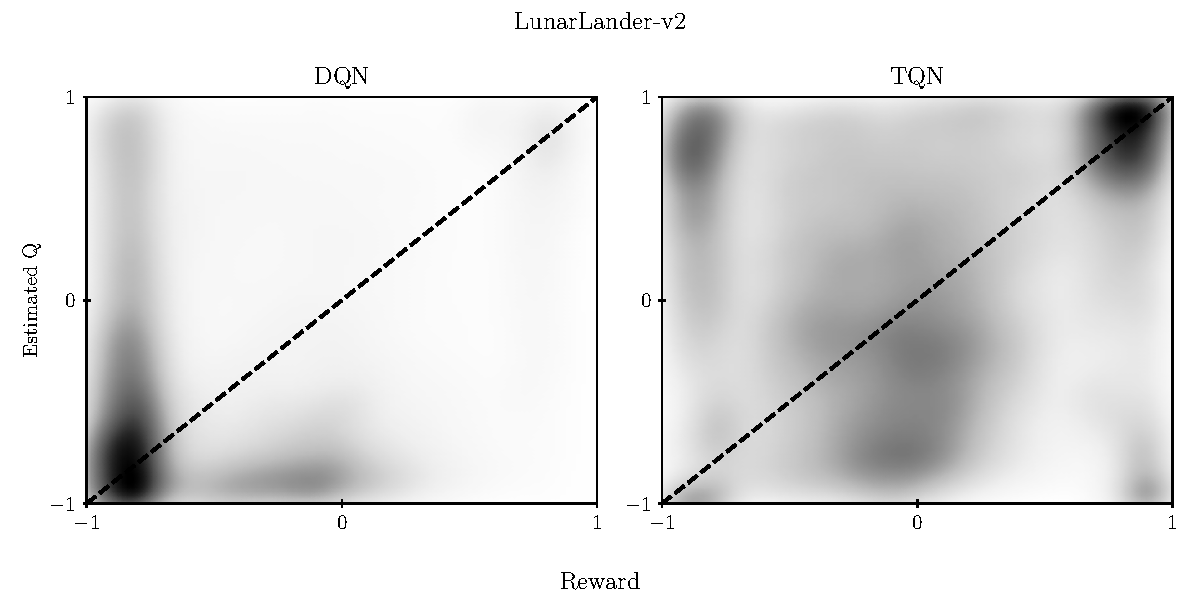
\includegraphics[width=\textwidth]{images/q-vs-reward_LunarLander-v2.pdf}
\caption{Density plot of the estimated Q-values versus environment step rewards sampled from $400$ episodes.}
\label{fig:q-vs-reward-LunarLander-v2}
\end{figure}

Despite the Q-values represent the overall confidence of the network while the step rewards are only an immediate feedback, it is still useful to visualize their relationship to better understand the behavior of the two architectures. As the rewards increase, the Q-values should also increase. Ideally, in \textbf{Fig.}~\ref{fig:q-vs-reward-LunarLander-v2}, the density should be aligned with the major diagonal. This would mean that Q-values estimates are well-aligned with the rewards each agent receives.

I can observe that, while both models present fluctuation, \acrshort{dqn} is more robust and it takes a more conservative approach; it is the most ``pessimistic" when it receives low rewards. The \acrshort{tqn} architecture instead is over-confident in its estimates and, although the model is most confident when it receives the highest rewards, as expected, it also shows a high degree of confidence when it receives the lowest rewards.

\begin{figure}[!htbp]
\centering
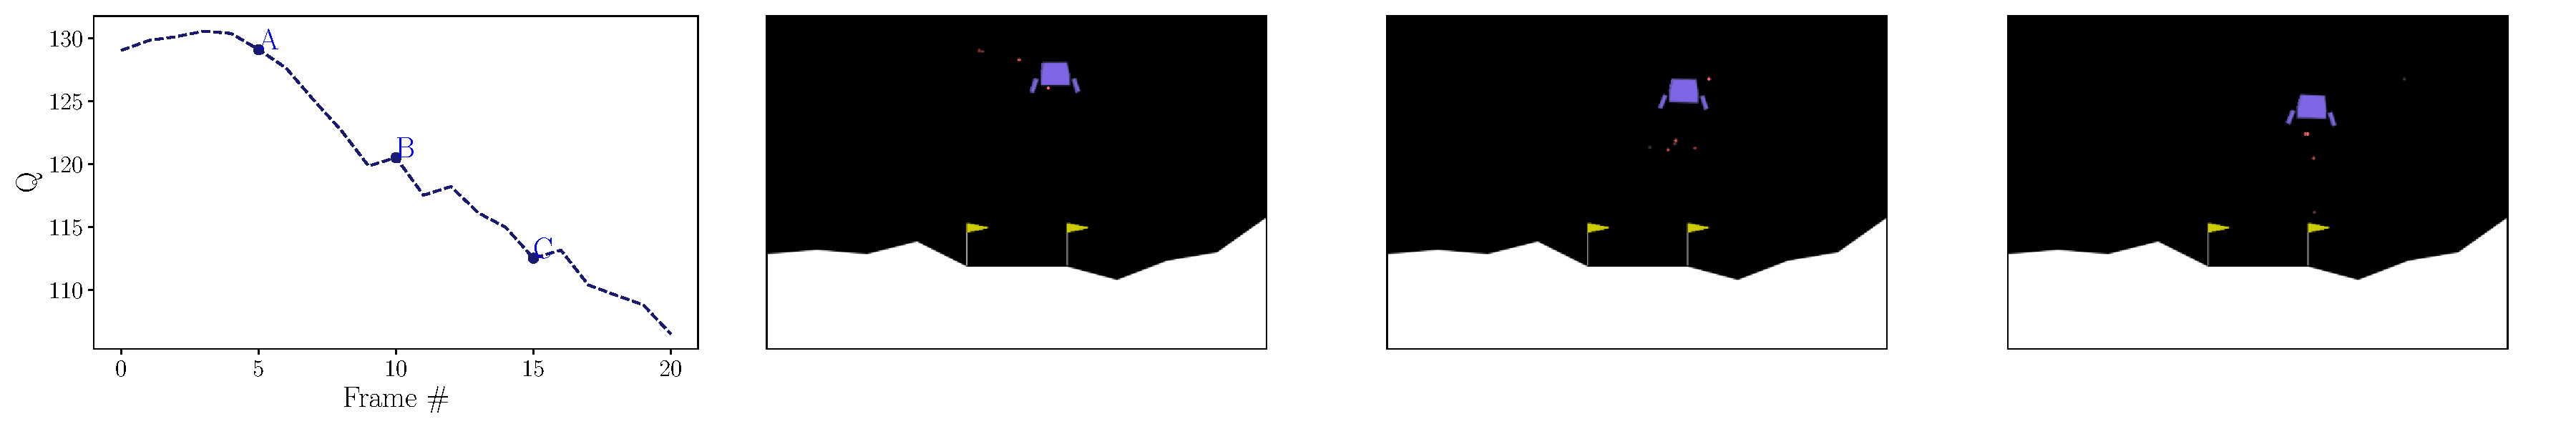
\includegraphics[width=\textwidth]{images/q-vs-frame_DQN_LunarLander-v2.pdf}
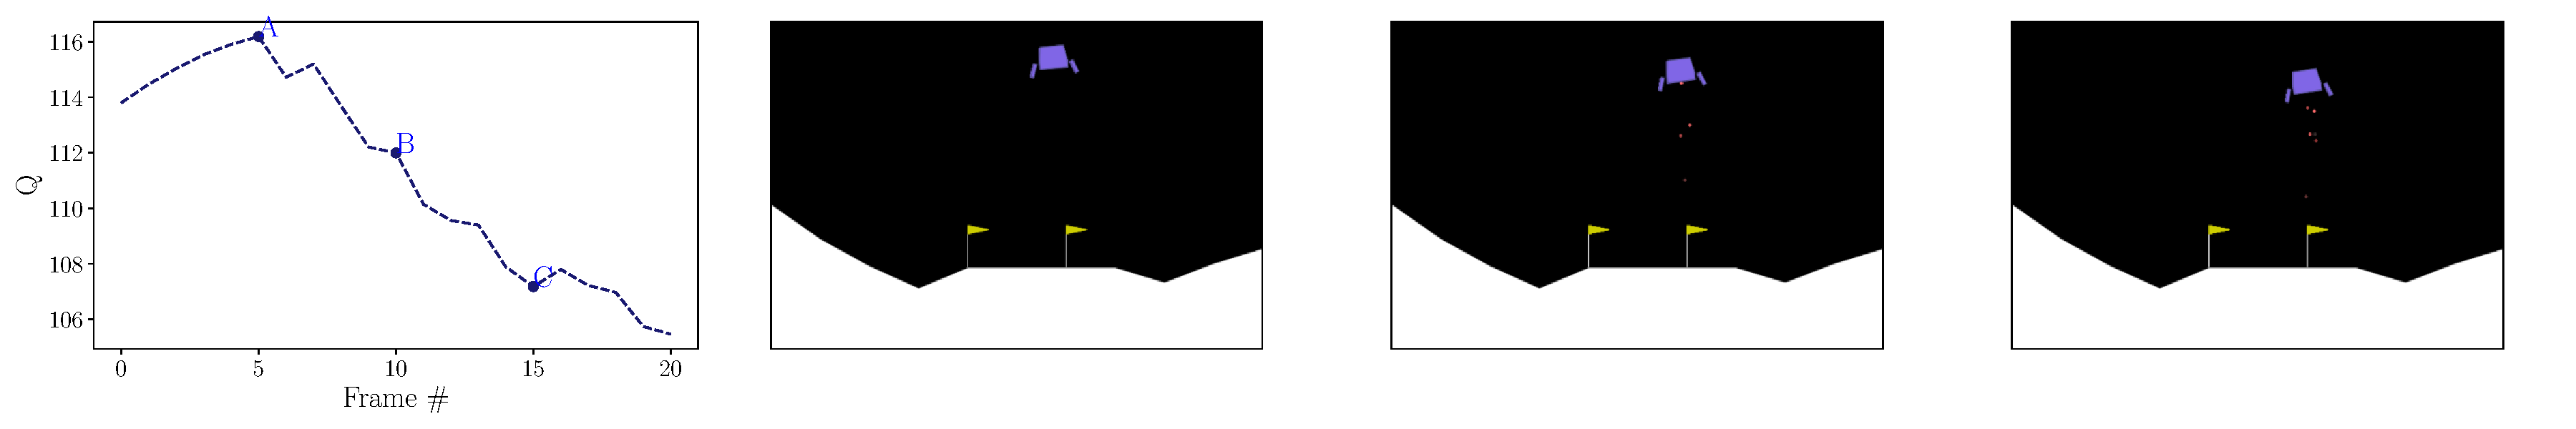
\includegraphics[width=\textwidth]{images/q-vs-frame_TQN_LunarLander-v2.pdf}
\caption{On the left, the predicted Q-values for a portion of a LunarLander episode. The three screenshots on the right correspond to the frames labeled by A, B, and C. The first row is from the \acrlong{dqn} and the second one from the \acrlong{tqn}.}
\label{fig:q-vs-screenshot-TQN-LunarLander-v2}
\end{figure}

Despite using a target network to dampen its confidence, \acrshort{tqn} is still prone to over-estimating Q-values. The over-confidence in the predictions matches what I show in \textbf{Fig.}~\ref{fig:q-vs-reward-LunarLander-v2}; the step of the loss function indicates that \acrshort{tqn} has learned steadily during training, but it has not fully converged yet.

\begin{figure}[!htbp]
\centering
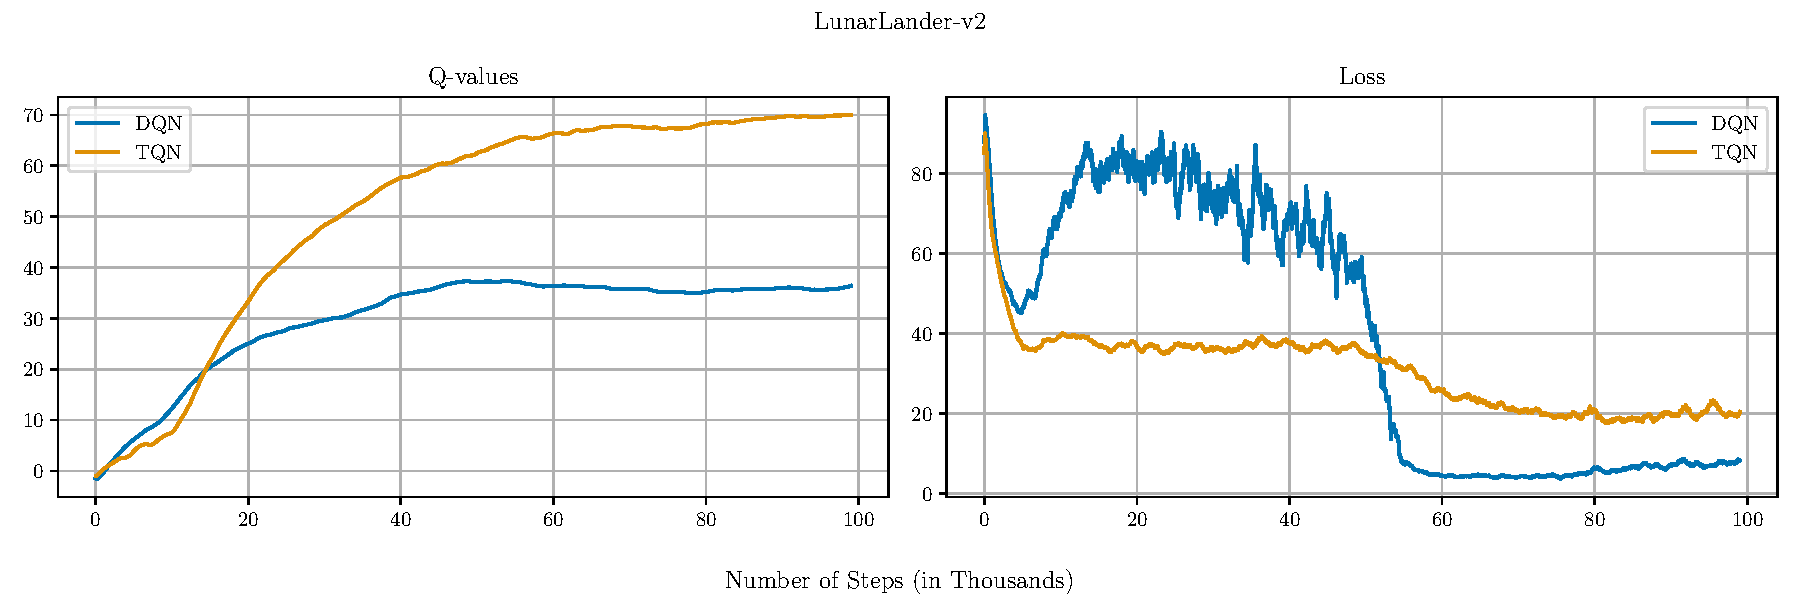
\includegraphics[width=\textwidth]{images/q-vs-loss_DQN-TQN_LunarLander-v2.pdf}
\caption{Q-values over time and loss over time. \acrshort{tqn} is over-confident and converges more slowly.}
\label{fig:q-vs-loss-LunarLander-v2}
\end{figure}

The last metrics (Fig.~\ref{fig:statistics-LunarLander-v2}) are again computed by normalizing the scores between $0$ and $\tau = 200$, the target score for which an episode of the LunarLander environment is considered successful (see \nameref{subsubsec:lunar_lander}). Albeit the magnitude is very small ($10^{-2}$), the \acrlong{tqn} is able to beat the baseline \acrshort{dqn} baseline. Large confidence intervals for the \textbf{median} mean that there are a few high performing tasks skewing the results and, to compensate for it, I choose the \acrshort{iqm}, explained above, as a better indicator of the performance \cite{rliable}. The \acrshort{iqm} is more robust than the mean to statistical outliers and, thanks to the smaller confidence intervals, it is able to detect improvements with fewer runs \cite{rliable}. As opposed to the probability of improvement, both the \acrshort{iqm} and the optimality gap that follows take into account the size of improvement.

\begin{figure}[!htbp]
\centering
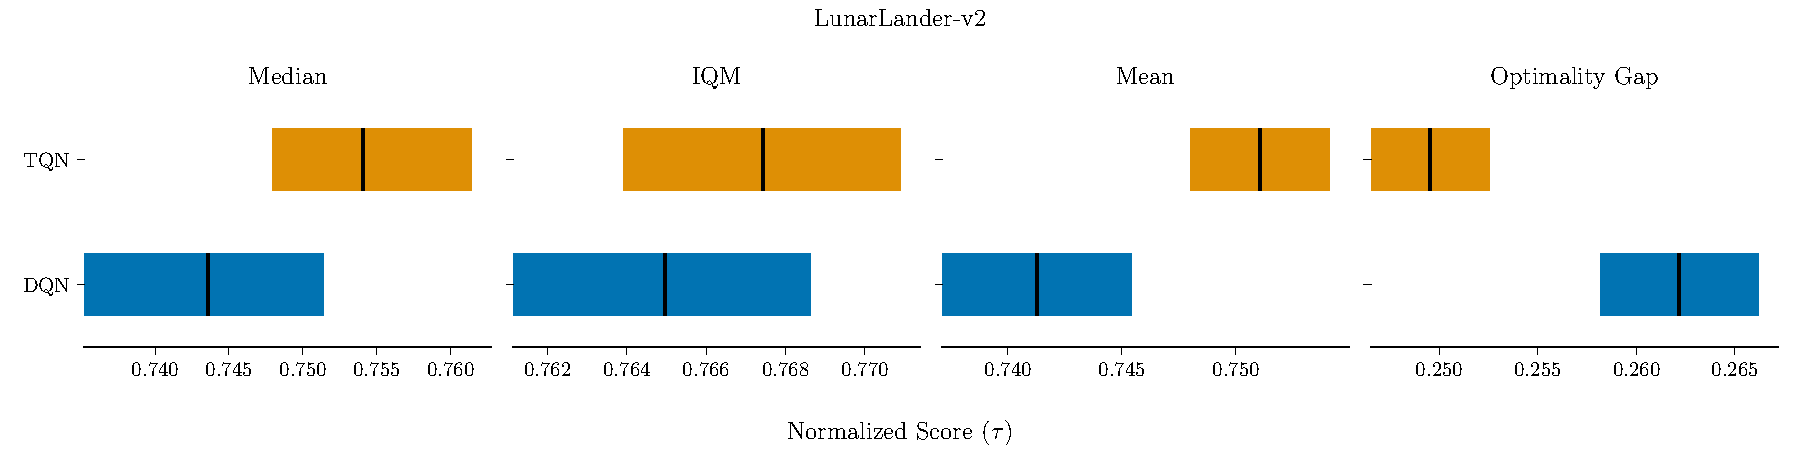
\includegraphics[width=\textwidth]{images/statistics_DQN-TQN_LunarLander-v2.pdf}
\caption{Aggregate metrics with 95\% confidence intervals.}
\label{fig:statistics-LunarLander-v2}
\end{figure}

Finally, a more robust alternative to the mean is the \textbf{optimality gap}, which is the amount by which the models fail to meet the target score $\tau$. The optimality gap assumes that scores above the threshold are less important than the rest. In this case a higher value corresponds to worse performance, and the results in \textbf{Fig.}~\ref{fig:statistics-LunarLander-v2} once again confirm that the novel architecture performs indeed better than the baseline.

\section{Conclusion}

I present an online \acrshort{rl} agent that can effectively learn from the environment by processing in parallel a sequence of transitions. I add a Transformer layer as a feature layer to a baseline double \acrshort{dqn} implementation and I show that the architecture is able to exploit information from the environment and to converge over time to the optimal policy.

To evaluate the \acrshort{tqn} against the baseline, I follow the approach first proposed by \cite{rliable}. Despite reusing the same set of hyperparameters with a different architecture, the new architecture is able to learn and beat the baseline on 1 out of the 3 environments.

As a first step for extra future work, performing a hyperparameter sweep is necessary. Hyperparameters that are optimal for \acrshort{dqn} may not be optimal for \acrshort{tqn} and vice versa; new ones are also introduced, such as the number of encoder and decoder layers, their size and the number of self-attention heads. It would also be interesting to study how the new architecture can be applied to physics environments that operate over continuous action spaces. In this case, adding a Transformer layer to a Deep Deterministic Policy Gradient (DDPG) may be trivial.

\section{Acknowledgements}

First of all, my thanks go to professor Vincent François-Lavet for his feedback and inputs during the trajectory of this paper and for having given me the opportunity to have a glimpse of what \acrshort{rl} research looks like; I look forward to contribute much, much more to the field. Then, in no particular order, I want to thank my whole family, my girlfriend Salomé for her unwavering love and support, and for her invaluable proof-reading skills, our cat Giulietta, who actually wrote all the code for this paper during feverish pair-programming sessions, my mother Maddalena, my father Girolamo and my sister Deborah for always being there.


\bibliographystyle{splncs04}
\bibliography{bibliography}

\section*{Appendix A: Reproducibility} \label{section:appendix_a}

\subsection*{Source Code}
Source code, trained models, logs, plots and other results are available at \url{https://github.com/robertoschiavone/transformer-q-network}.

\subsection*{Seeds}
Every data point is collected using 20 different seeds, from 1693526400 to 1695168000, with increments of 86400 between them. Each seeds represents the Unix time from September 1, 2023 00:00:00 GMT to September 20, 2023 00:00:00 GMT. The seeds are chosen for no specific reason other than ensuring the reproducibility of the results. The final list of seeds is

\begin{verbatim}
seeds = [ 1693526400, 1693612800, 1693699200, 1693785600, 1693872000,
          1693958400, 1694044800, 1694131200, 1694217600, 1694304000,
          1694390400, 1694476800, 1694563200, 1694649600, 1694736000,
          1694822400, 1694908800, 1694995200, 1695081600, 1695168000 ].
\end{verbatim}

\section*{Appendix B:  Self Reflection} \label{section:appendix_b}

I started the project with a high degree of confidence about my knowledge of \acrlong{rl}, and the original starting point was the grandiose idea of training a single agent (not even a single architecture!) capable of playing all Atari games.
I have learned that good research takes time, and it is not feasible to test all variants of plausible solutions on every environment ever published. Time acts as a strainer that filters out the irrelevant details and lets you focus on the important parts of the work.

During my research, I have come to realize that yes, this paper will show how much I know about \acrshort{ai} and \acrshort{rl}, but also that my knowledge is extremely narrow and limited, and \textbf{this is fine}. The field of \acrshort{rl} is vast and it is thriving thanks to a fresh stream of interesting concepts and ideas, and I would need more than a lifetime to master and keep up with everything that has been published so far. I have found my niche though, with its engaging set of problems, growing at each discovered solution, puzzles whose original pictures are missing and all their pieces are scrambled.

\section*{Appendix C: Additional Experiments} \label{section:appendix_c}

\subsection*{Acrobot}

While the baseline works as expected, \acrshort{tqn} is not able to converge. Despite the score starts to weakly increase, the loss is still growing over time. All metrics further prove that the \acrlong{tqn} is far from reaching an optimal policy.

\begin{figure}[!htbp]
\centering
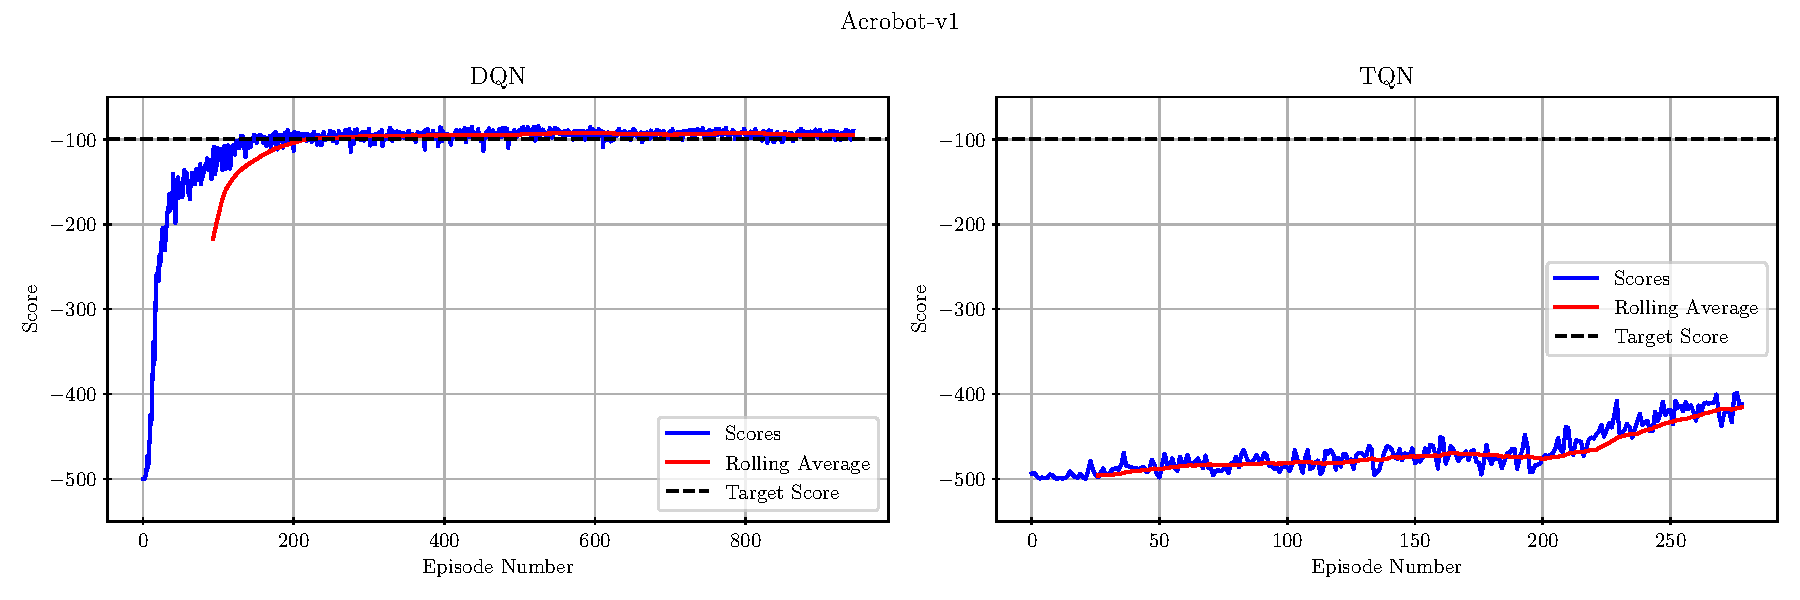
\includegraphics[width=\textwidth]{images/score-vs-episode_DQN-TQN_Acrobot-v1.pdf}
\caption{Score trend over time during training for Acrobot.}
\label{fig:score-vs-episode-Acrobot-v1}
\end{figure}

\begin{figure}[!htbp]
\centering
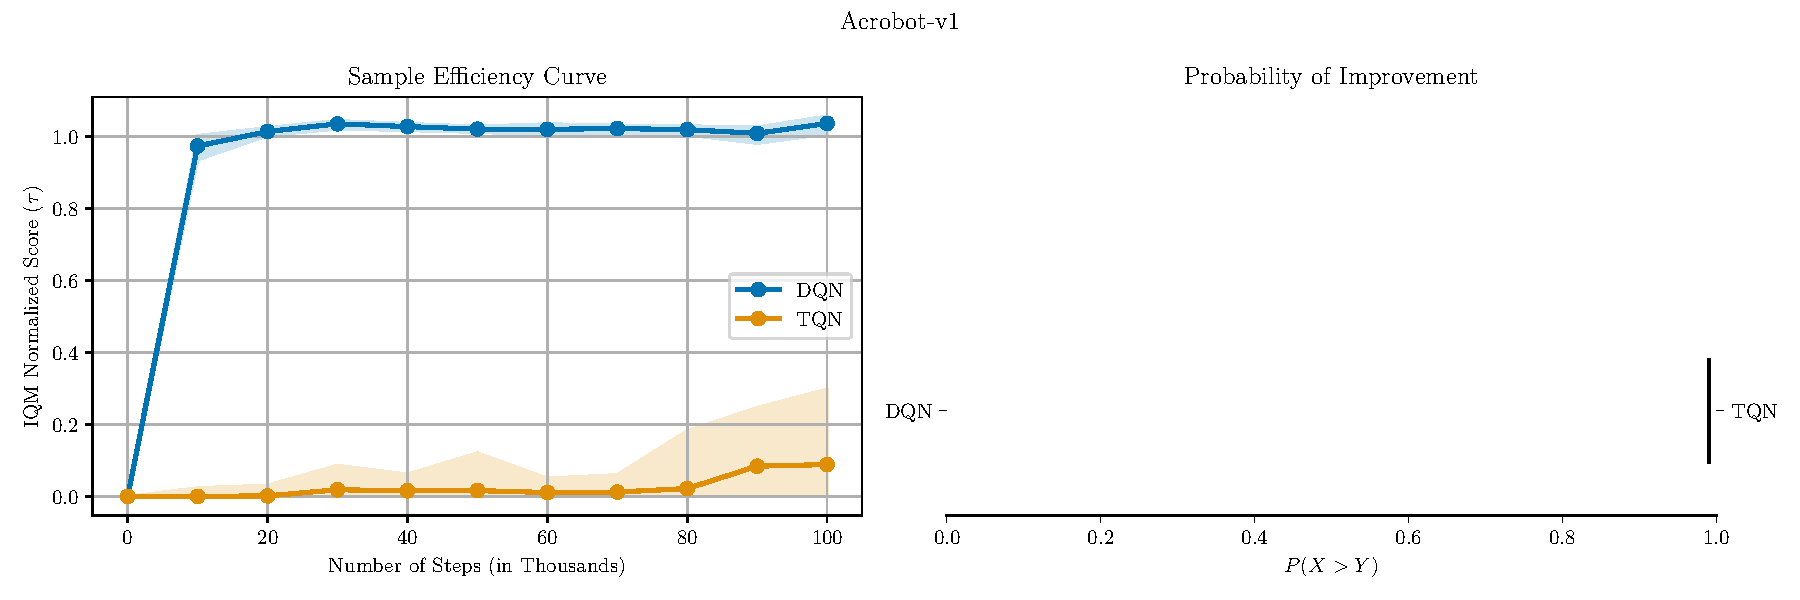
\includegraphics[width=\textwidth]{images/sample-efficiency-probability-improvement_DQN-TQN_Acrobot-v1.pdf}
\caption{Sample efficiency and probability of improvement for Acrobot.}
\label{fig:sample-efficiency-Acrobot-v1}
\end{figure}

\begin{figure}[!htbp]
\centering
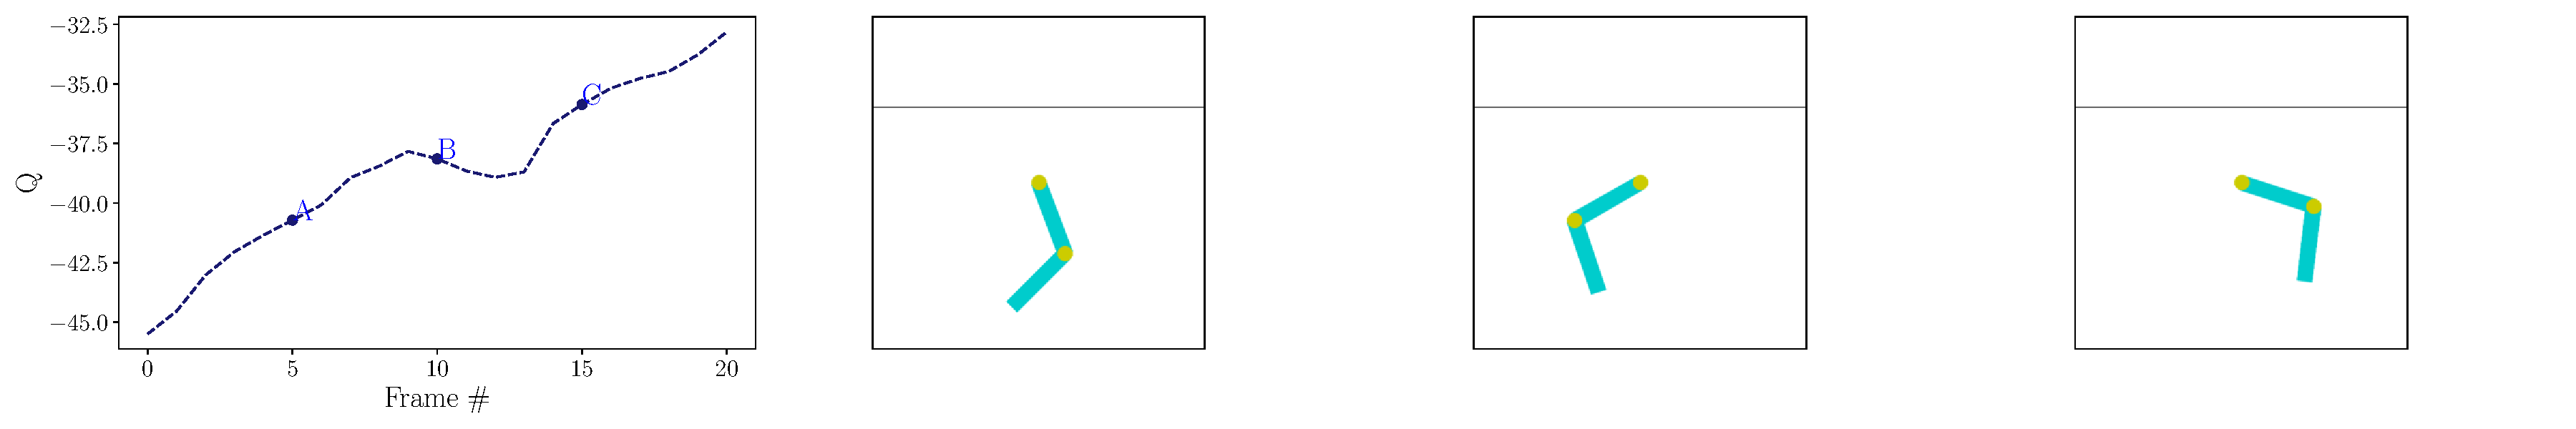
\includegraphics[width=\textwidth]{images/q-vs-frame_DQN_Acrobot-v1.pdf}
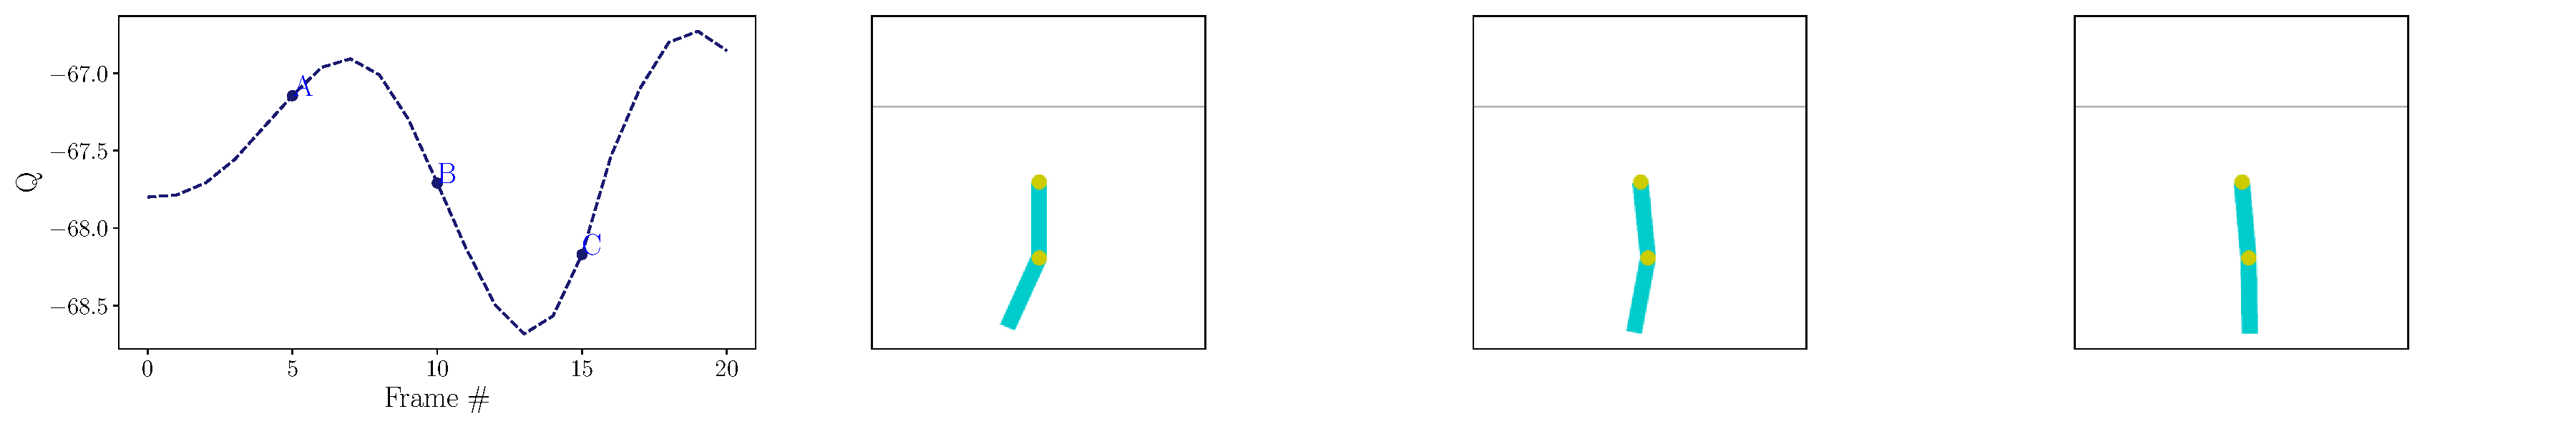
\includegraphics[width=\textwidth]{images/q-vs-frame_TQN_Acrobot-v1.pdf}
\caption{The predicted Q-values for a portion of a Acrobot episode and the three screenshots corresponding to frames A, B, and C. From top to bottom: \acrshort{dqn} and \acrshort{tqn}.}
\label{fig:q-vs-frame-DQN-Acrobot-v1}
\end{figure}

\begin{figure}[!htbp]
\centering
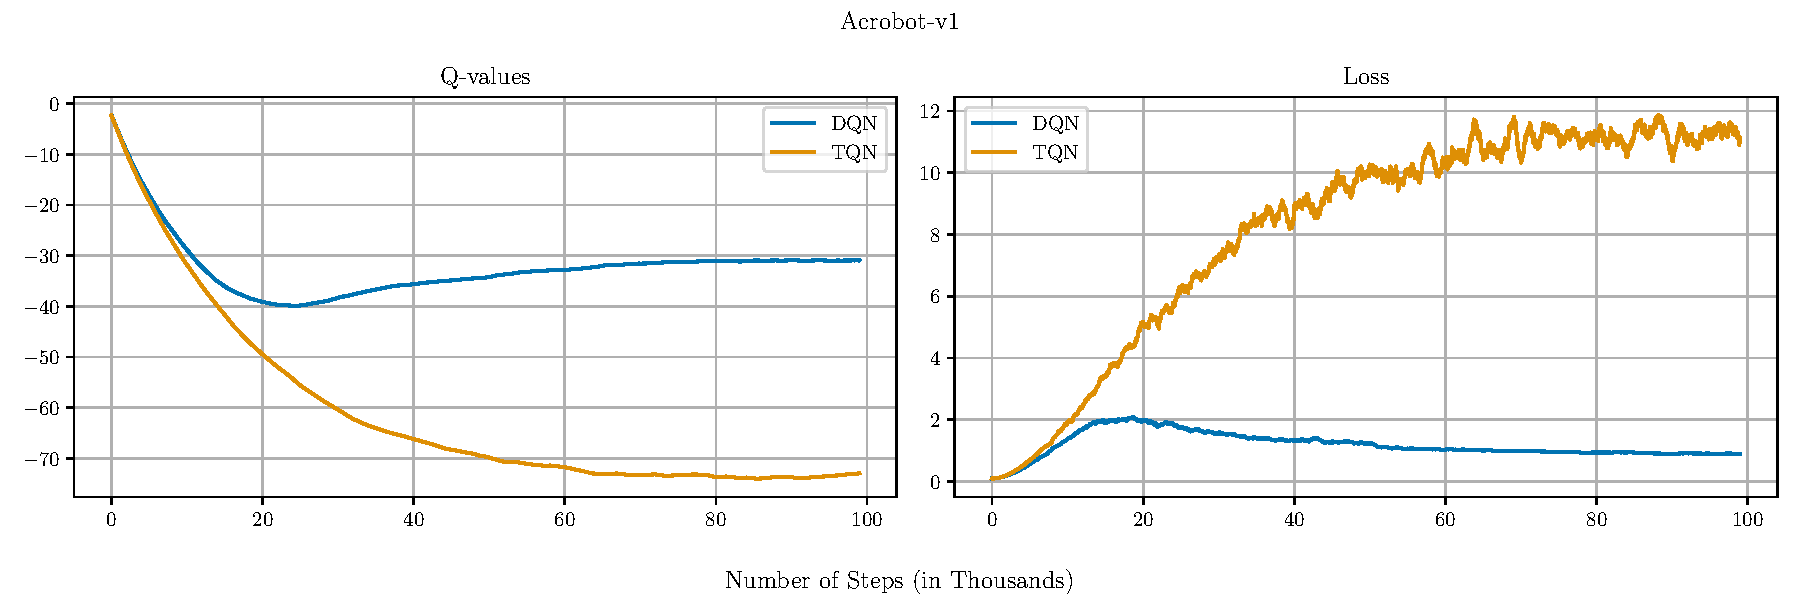
\includegraphics[width=\textwidth]{images/q-vs-loss_DQN-TQN_Acrobot-v1.pdf}
\caption{Q-values and loss over time for Acrobot.}
\label{fig:q-vs-loss-Acrobot=v1}
\end{figure}

\begin{figure}[!htbp]
\centering
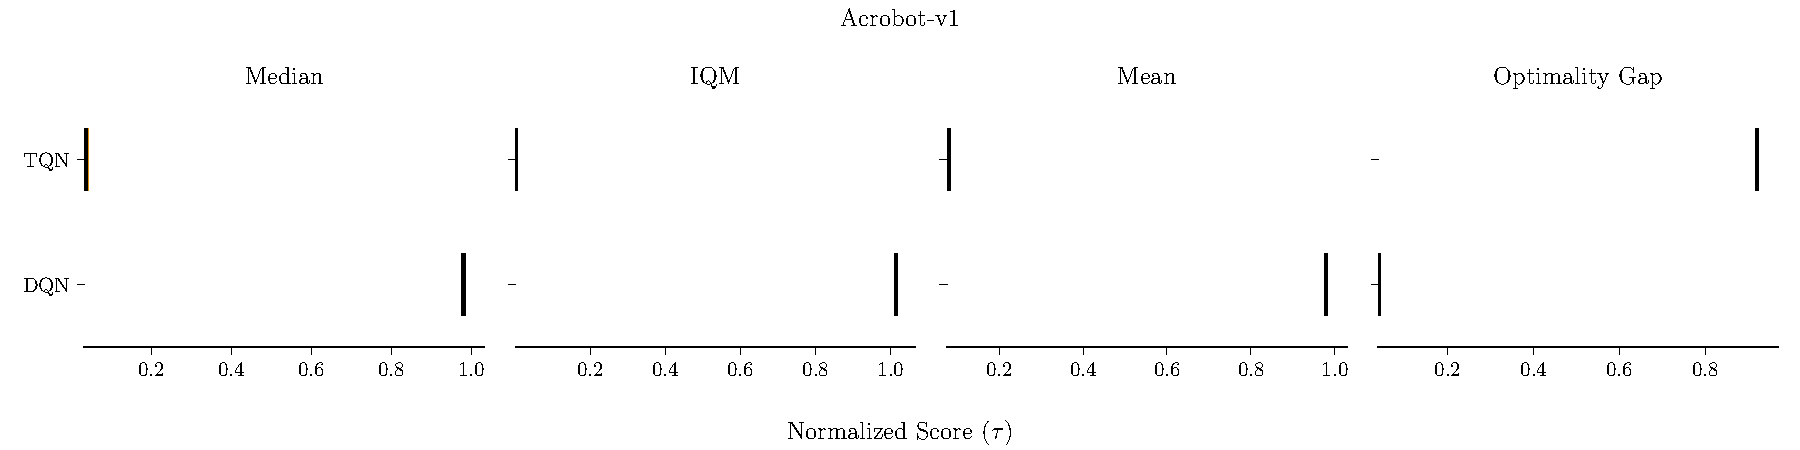
\includegraphics[width=\textwidth]{images/statistics_DQN-TQN_Acrobot-v1.pdf}
\caption{Median, \acrshort{iqm}, mean and optimality gap for Acrobot.}
\label{fig:statistics-Acrobot-v1}
\end{figure}

\subsection*{CartPole}
CartPole is widely regarded as one of the simplest environments, and yet no architecture was able to learn in the given amount of steps. There may be some differences with the implementation from which I borrow the hyperparameters \cite{rl_zoo3} that do not allow the agent to learn, or the hyperparameters are not really optimal and need further tuning. Time was limited though, and I was not able to further investigate the problem.

\begin{figure}[!htbp]
\centering
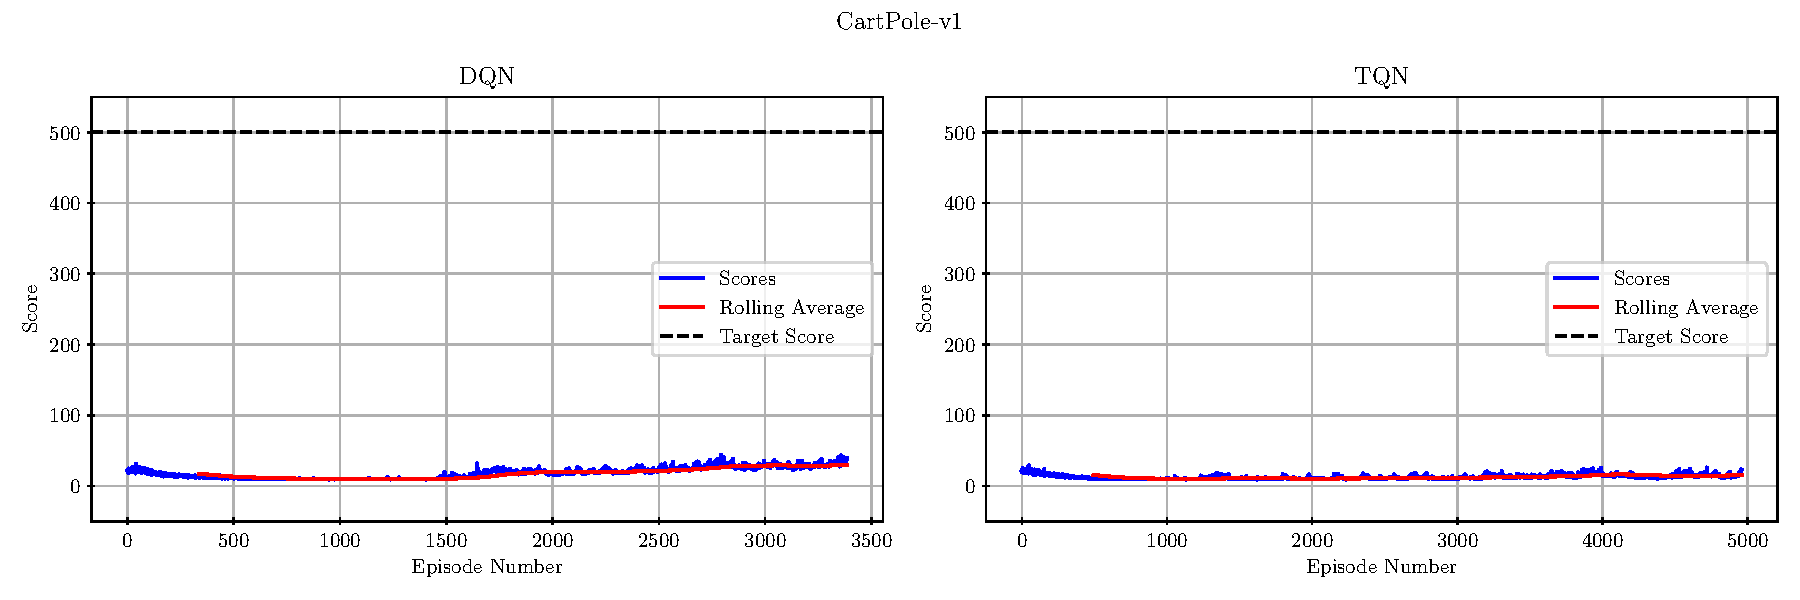
\includegraphics[width=\textwidth]{images/score-vs-episode_DQN-TQN_CartPole-v1.pdf}
\caption{Score trend over time during training for CartPole.}
\label{fig:score-vs-episode-CartPole-v1}
\end{figure}

\begin{figure}[!htbp]
\centering
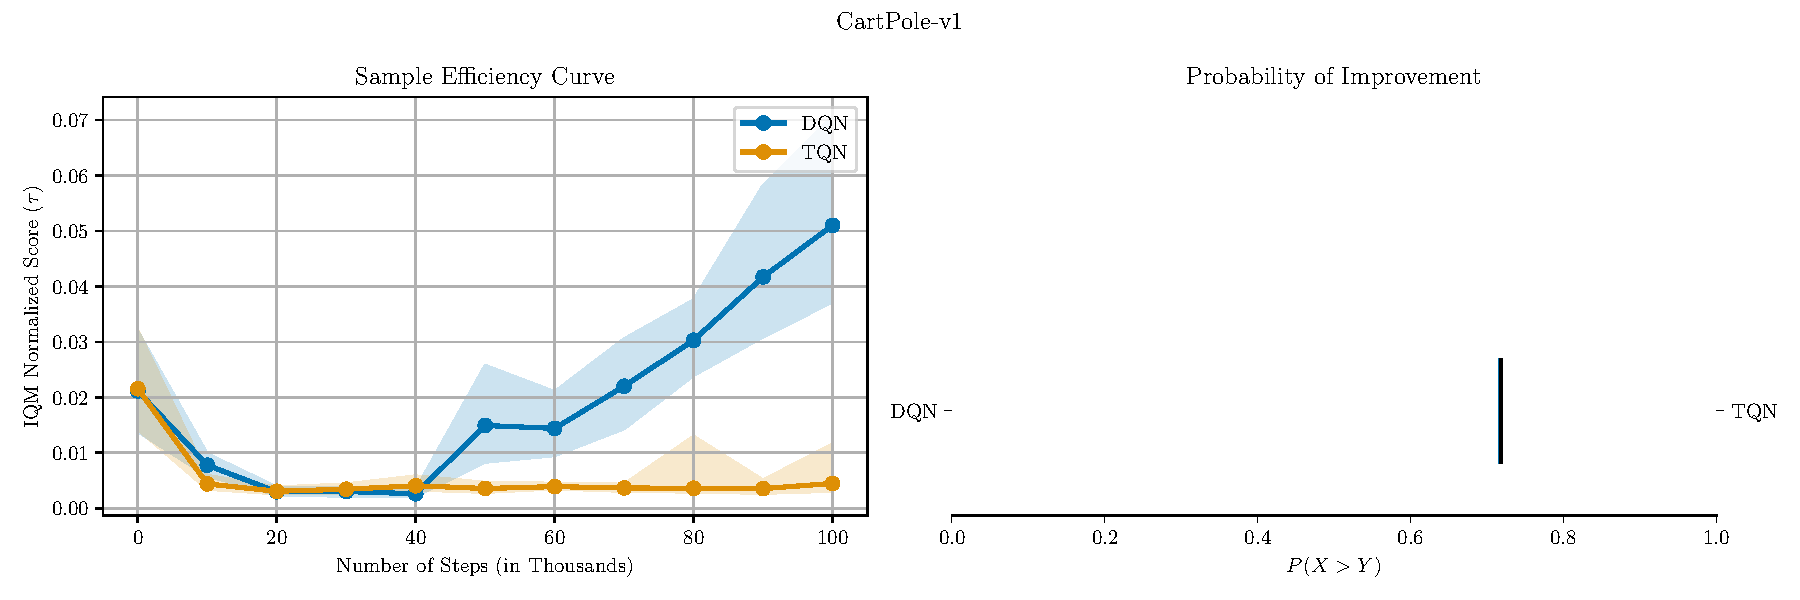
\includegraphics[width=\textwidth]{images/sample-efficiency-probability-improvement_DQN-TQN_CartPole-v1.pdf}
\caption{Sample efficiency and probability of improvement for CartPole.}
\label{fig:sample-efficiency-CartPole-v1}
\end{figure}

\begin{figure}[!htbp]
\centering
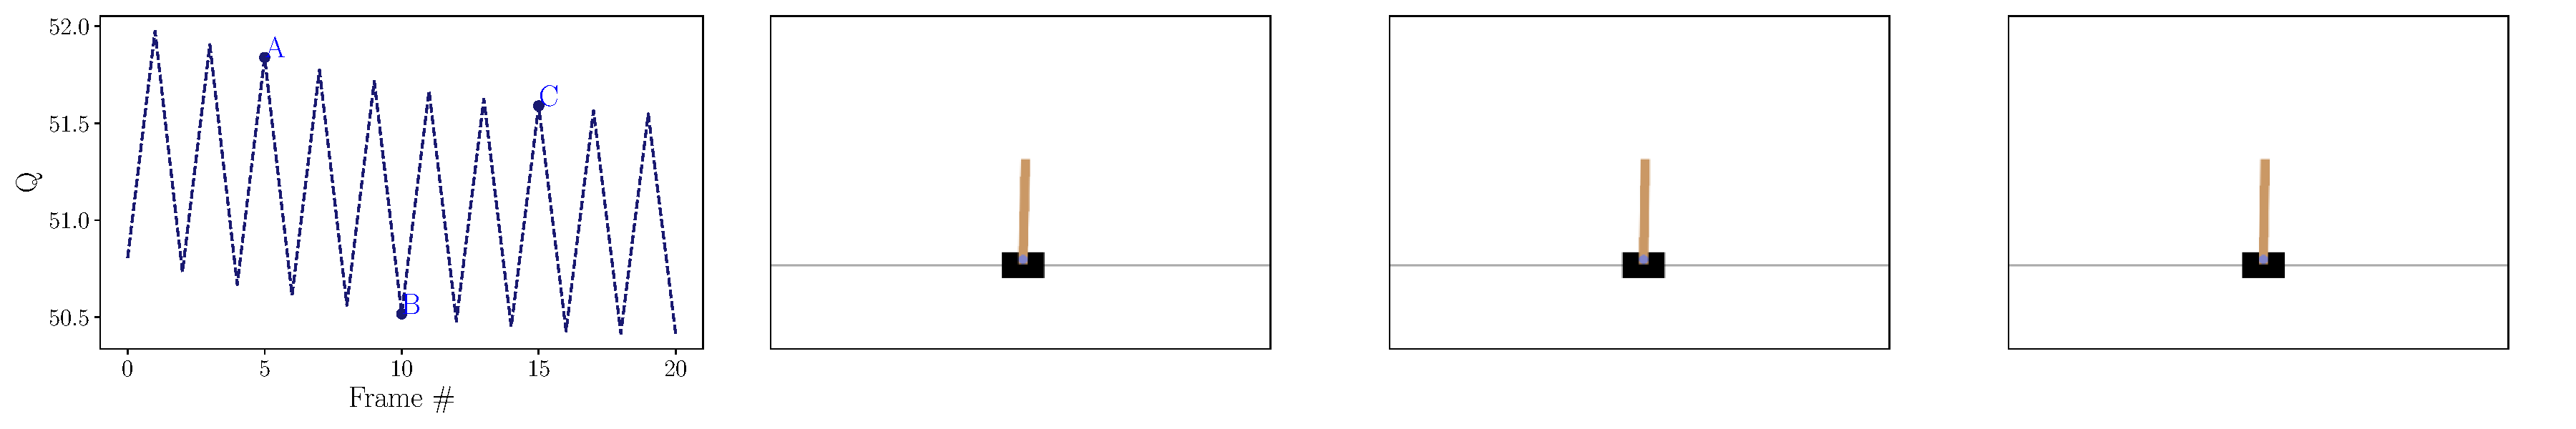
\includegraphics[width=\textwidth]{images/q-vs-frame_DQN_CartPole-v1.pdf}
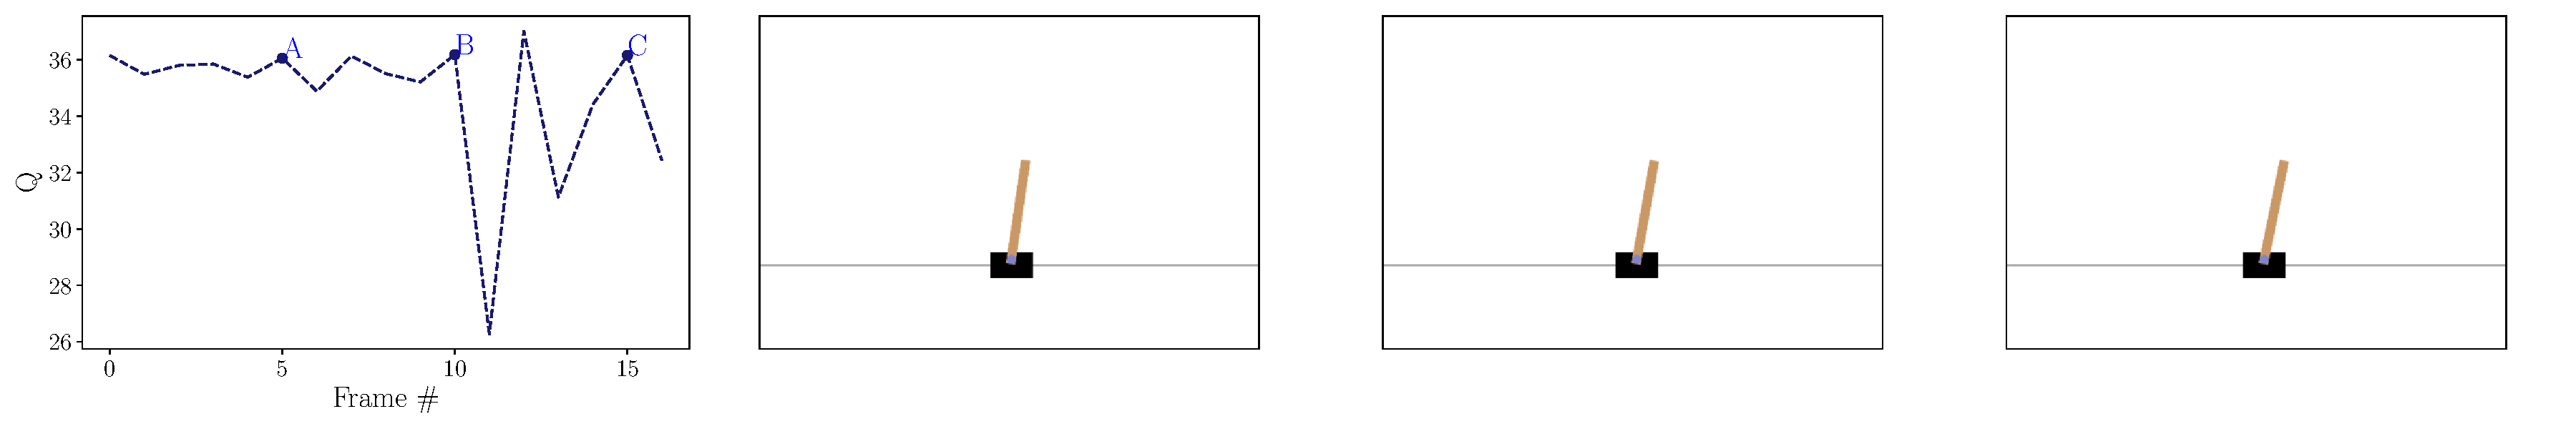
\includegraphics[width=\textwidth]{images/q-vs-frame_TQN_CartPole-v1.pdf}
\caption{The predicted Q-values for a portion of a CartPole episode and the three screenshots corresponding to frames A, B, and C. From top to bottom: \acrshort{dqn} and \acrshort{tqn}.}
\label{fig:q-vs-frame-DQN-CartPole-v1}
\end{figure}

\begin{figure}[!htbp]
\centering
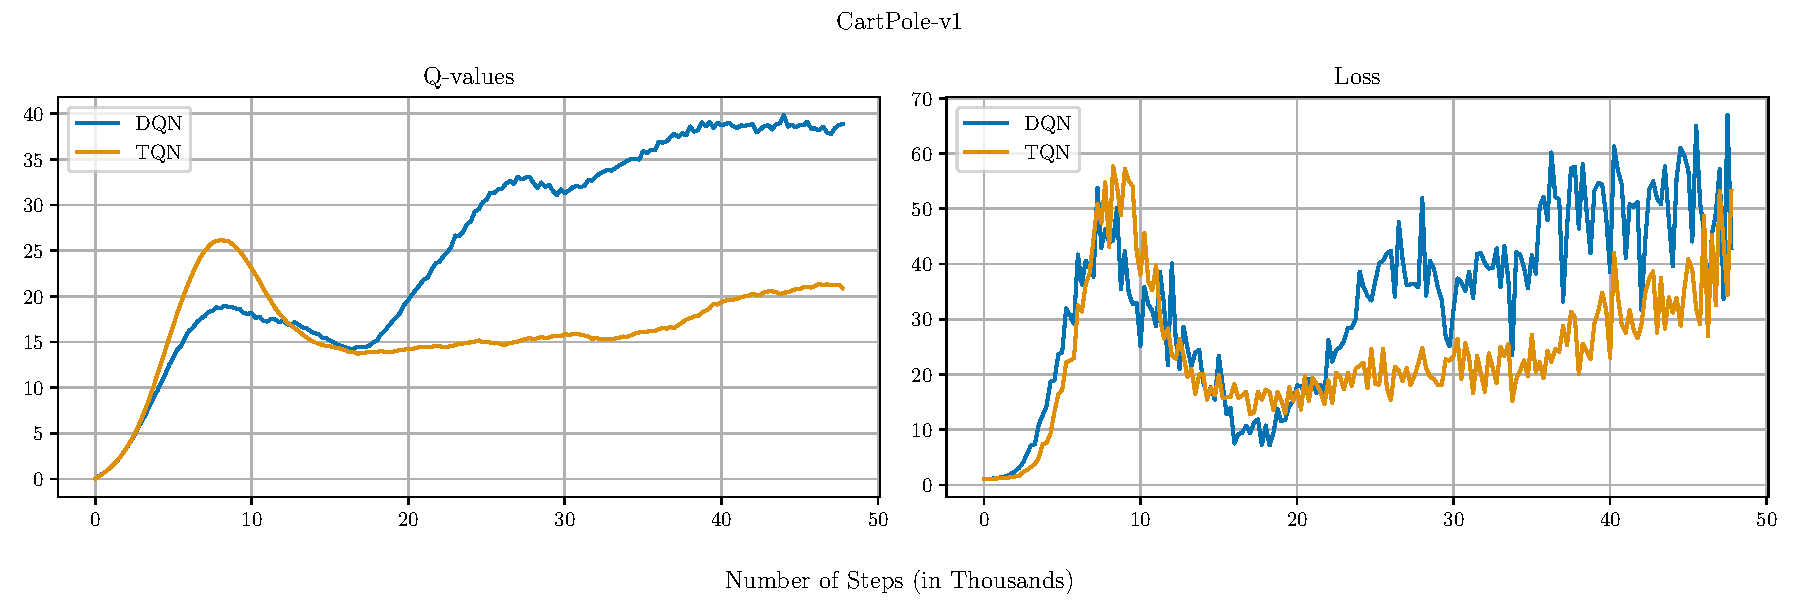
\includegraphics[width=\textwidth]{images/q-vs-loss_DQN-TQN_CartPole-v1.pdf}
\caption{Q-values and loss over time for CartPole.}
\label{fig:q-vs-loss-CartPole-v1}
\end{figure}

\begin{figure}[!htbp]
\centering
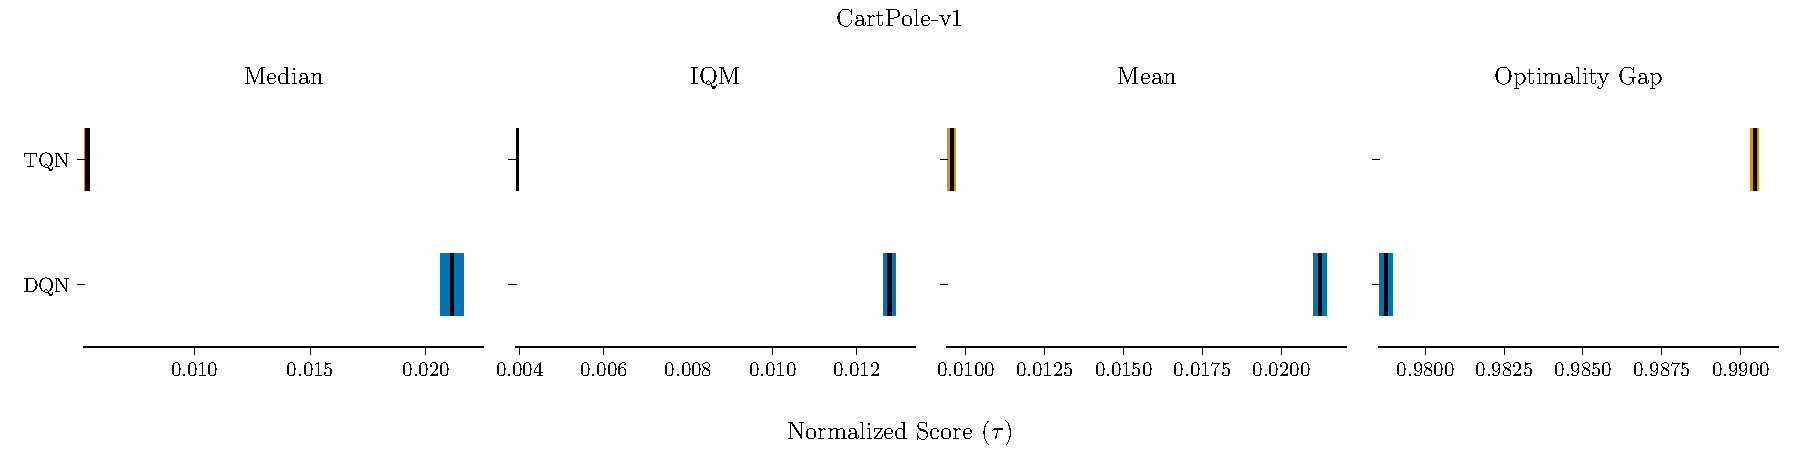
\includegraphics[width=\textwidth]{images/statistics_DQN-TQN_CartPole-v1.pdf}
\caption{Median, \acrshort{iqm}, mean and optimality gap for CartPole.}
\label{fig:statistics-CartPole-v1}
\end{figure}


\printglossary[type=\acronymtype]

\end{document}
